% Introduction part II
This part of the thesis will present the work done in our specialization project before and leading up to the master thesis period. It is the foundation for inventing and developing our chosen concept Hover. First, an introduction to general game development concepts is given. Specifically, how to design an enjoyable game, player types, and game reward systems. After that, a definition, common characteristics, and a description of existing alternative games are presented. Further on, a technology review exploring the possibilities in alternative games’ field and relevant technologies is conducted. At last, all the potential concepts we invented during the specialization project conclude the part.
\clearpage

\section{Design an Enjoyable Game}
\label{chap:design_an_enjoyable_game}

How to create an enjoyable game is an important part of every game development process. This chapter presents a literature study of the subject based on work conducted by \citeauthor{malone_what_1980} in \citeyear{malone_what_1980}, and \citeauthor{sweetser_gameflow_2005}’s “GameFlow: a model for evaluating player enjoyment in games” article. \citeauthor{malone_what_1980}’s research outlines challenge, fantasy, and curiosity as the three main elements to increase motivation in games. The GameFlow article presents a model for evaluating enjoyment in games based on eight elements. Even though different authors wrote these articles, they present a lot of the same mindset in what characterizes an enjoyable game.

\subsection{What Makes Things Fun to Learn?}
Malone presented in his study from \citeyear{malone_what_1980} a framework for creating enjoyable games. As mentioned above, he organized the essential properties of what makes a good game into the three categories—challenge, fantasy, and curiosity. Malone wrote multiple articles on the topic. His main findings were summarized in “What Makes Things Fun to Learn? Heuristics for Designing Instructional Computer Games”. Even though this research was conducted in 1980 and the examples he presents are somewhat old, the main concepts are still highly relevant today.

\subsubsection{Challenge}
The first property presented by Malone is \textit{challenge}:

\blockquote{In order for a computer game to be challenging, it must provide a goal whose attainment is uncertain.} \citep{malone_what_1980}. 

From this principle, three essential characteristics of why challenge is necessary to create good computer games follow:

\textbf{Goal} \\
Based on studies done by Malone, users tend to prefer games that have clearly defined goals. However, it is necessary to note that all goals are not equally valuable. Consequently, four different properties on how to create appropriate goals are mentioned:

\begin{enumerate}
    \item Simple games should include obvious goals.
    \item A complex environment should provide a structure so that players can easily generate appropriately difficult goals.
    \item Practical and fantasy goals are often the best ones.
    \item Players need to know when they are getting closer to the goal.
\end{enumerate}

\textbf{Uncertain outcome} \\
The next characteristic is \textit{uncertain outcome}, and the article describes four different ways  it can make computer games more challenging:

\begin{enumerate}
    \item \textbf{Variable difficulty levels}\\ 
    Good computer games should include variable difficulty levels that can match the user’s skill level. The difficulty level can be determined in three ways: Automatically, chosen by the player, or determined by the opponent’s skills.
    \item \textbf{Multiple level goals} \\ 
    Finding a goal for various player types is easier when creating multiple-level goals. Generally, two levels of goals are defined: Basic goals and meta goals. One typical example of this could be to have a basic goal of completing platform game levels. Collecting all the coins could then be the meta-goal. 
    \item \textbf{Hidden information} \\
    Hiding information can be an appropriate way of creating challenging games. Guessing games use this technique regularly.
    \item \textbf{Randomness} \\
    One last way of creating challenging games is to include randomness. When a random element is included, the player cannot predict the next step, making the game more challenging. Gambling games primarily succeed based on using randomness.
\end{enumerate}

\textbf{Self-esteem} \\
In addition to goals and uncertain outcomes, self-esteem is mentioned in the article. Self-esteem can be seen as the reason why goals and challenges are essential in good games. Completing goals and challenges can increase a person’s self-esteem and thus create a captivating game.

\subsubsection{Fantasy}
The next property is fantasy, which is often used in games to make them more appealing. In games, fantasies often appear as models of physical objects and social settings that are not truly present \citep{malone_what_1980-1}.

One typical example where fantasy is used to increase enjoyment is in learning games, where one can increase the level of fun by overlaying the curriculum with elements of fantasy. The fantasy can visualize the progression of the player towards the goal based on right or wrong answers. An example could be getting to the finish line in a marathon or avoiding a catastrophe, like in Hangman. In these games, the fantasy depends on how the skill is used, but not necessarily vice versa. Fantasies that only have the one-way logical dependency, where skill affects the fantasy, are called extrinsic fantasies. Extrinsic fantasies are good for arithmetic problems, where answers are either wrong or right, and the skill does not depend on the fantasy \citep{malone_what_1980}.

\begin{figure}[H]
    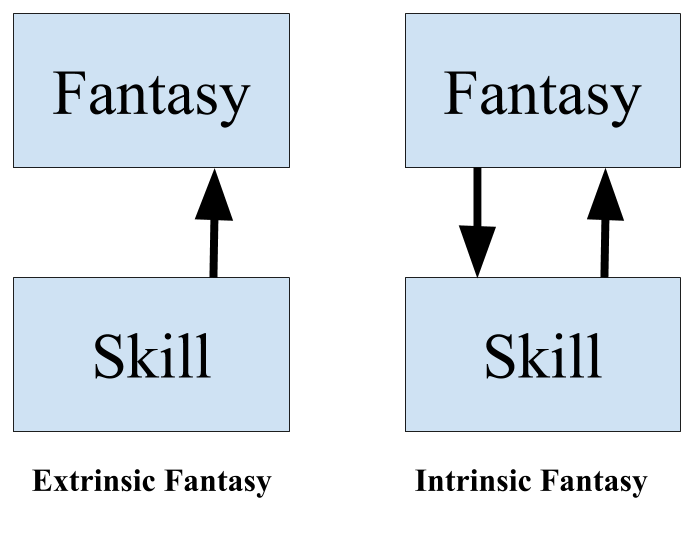
\includegraphics[width=0.5\textwidth]{Images/Theory/SkillFantasy.png}
    \centering
    \caption{Logical dependencies in extrinsic and intrinsic fantasies \citep{malone_what_1980}.}
    \label{fig:skill_fantasy}
\end{figure}

Fantasies that have a two-way logical dependency are named intrinsic fantasies; the fantasy depends on the skill, and the skill depends on the fantasy. Figure \ref{fig:skill_fantasy} illustrates the two types of fantasy side-by-side. In the spelling game Hangman, the player’s spelling skills affect the fantasy, and the feedback of right or wrong guesses from the fantasy influences the player's skill as it becomes easier to guess new letters each time.

\textbf{The emotional aspect of fantasy} \\
Fantasies in games can appeal to players differently based on what emotions they need to satisfy \citep{malone_what_1980}. It may be challenging to design a computer game that meets the emotional needs of the person playing. Malone states that “... fantasies can be very important in creating intrinsically motivating environments but that, unless the fantasies are carefully chosen to appeal to the target audience, they may actually make the environment less interesting rather than more.” \citep{malone_heuristics_1982}. This statement suggests that different people find different fantasies appealing and that the fantasy must be appropriate for the target audience. Furthermore, if games had different fantasies to choose between, players are more likely to find it enjoyable, motivating, and engaging because it has a broader appeal.

\subsubsection{Curiosity}
The last property, curiosity, is about a player’s motivation to learn within a game environment. The learning is, however, independent from goal-seeking or fantasy-fulfillment. Games can trigger a player's curiosity by creating optimal information complexity environments based on their existing knowledge. Finding such balance for the information complexity will evoke the player’s curiosity to explore the environment further. An optimal environment has a complexity level where the player uses its knowledge to create an expectation of how the environment should behave. Still, these expectations should sometimes be unmet to be novel and introduce an element of surprise. Malone states curiosity should be distinguished into two categories: sensory and cognitive.

\textbf{Sensory curiosity} \\
Sensory curiosity is about the use of sensory-stimulating technology that attracts the user’s attention. In games, sensory curiosity appears as both audio or visual effects. Malone suggests that the effects can be used in four main ways \citep{malone_what_1980}:

\begin{enumerate}
    \item \textbf{As decoration} \\
    The use of audio and visual effects that are present regardless of user interactions. In games like Just Dance Now, this can be found as background music in the menu.
    \item \textbf{For enhancing fantasy} \\
    Sensory curiosity is used to improve fantasy in a game like “decorative” effects. However, the special effects are distinguishable because of their captivating nature and association with fantasy. In Wii Fit, this appears as audio effects that mimic an audience.
    \item \textbf{As a reward} \\
    The use of audio and graphical effects to reward good performance. It can increase the motivation for reaching the goal. Pokémon Go uses flashing lights and stars, together with victory sound, when users perform well, for instance, when they catch a new Pokémon.
    \item \textbf{As a representation system} \\
    Is the use of audio and visuals to convey information without using text. This usage is widely used in games to share information with the user efficiently. If a player in Pokémon Go unsuccessfully throws a Pokéball at a Pokémon, then the Pokéball will bounce away to indicate that a player missed the Pokémon.
\end{enumerate}

\textbf{Cognitive curiosity} \\
Cognitive curiosity is about the desire to improve one’s knowledge structures. Malone claims that people prefer their cognitive structures to be complete, consistent, and parsimonious. According to his theory, to stimulate a player’s cognitive curiosity, they must be given just enough information to make their existing knowledge appear incomplete, inconsistent, or miserly. Cognitive curiosity will engage the user because people are willing to learn more to improve their knowledge-structures. A typical example occurs when people are watching a movie with only some minutes left. The probability of them watching the rest of the video is high because they want to figure out how it will end and bring completeness to their knowledge structure.

\subsection{GameFlow}
Another essential framework for creating good games is \citeauthor{sweetser_gameflow_2005}’s “GameFlow: A Model for Evaluating Player Enjoyment in Games“ from \citeyear{sweetser_gameflow_2005}. The authors define a model for designing, evaluating, and understanding enjoyment in games based on work previously done by \citeauthor{csikszentmihalyi_flow_1990} in 1990. \citeauthor{csikszentmihalyi_flow_1990} conducted extensive research and surveys to find out what makes experiences enjoyable. Sweetser and Wyeth modified these principles to be representative of enjoyment in games. The GameFlow model consists of eight elements—concentration, challenge, skills, control, clear goals, feedback, immersion, and social interaction. Each of these includes a goal and a set of criteria that can be used when developing games \citep{sweetser_gameflow_2005}.

\subsubsection{Concentration}
Concentration is the first of the eight elements presented in the article. Enhancing how much concentration a task requires increases its immersion. Games should grab the player’s attention immediately and keep holding it for as long as possible. The player’s workload should be maintained at an appropriate level, and unimportant tasks should not be presented during the game to achieve this. Also, nongame-related interactions (e.g., settings menu) should be minimized, and the game should strive to use as much screen real estate  as possible for the gameplay. 

In Guitar Hero, players have to stay highly concentrated throughout the game. The gameplay is set in an environment with few distractions so that the player can become more immersed. The game also forces the player to stay concentrated throughout the song to avoid ending up in the game-over state. Figure \ref{fig:guitar_hero_gameplay} illustrates a screenshot from the gameplay in Guitar Hero.

\begin{figure}[H]
    
\includegraphics[width=0.8\textwidth]{Images/Theory/GuitarHeroGameplay.jpg}
    \centering
    \caption{Screenshot of gameplay in Guitar Hero.}
    \label{fig:guitar_hero_gameplay}
\end{figure}

\subsubsection{Challenge}
Challenge is often considered the essential aspect of good game design, and appropriate challenges should be presented to the player. The players’ skill levels should match the challenges given. Additionally, the challenge level should increase as the player moves through the game at an appropriate pace. In the language learning game Duolingo, players take a placement test to start at a proper level of challenge, as seen in Figure \ref{fig:dulingo_placement_test}. This test makes sure that any previous language experience is considered to match the player’s skill to the level of difficulty.

\begin{figure}[H]
    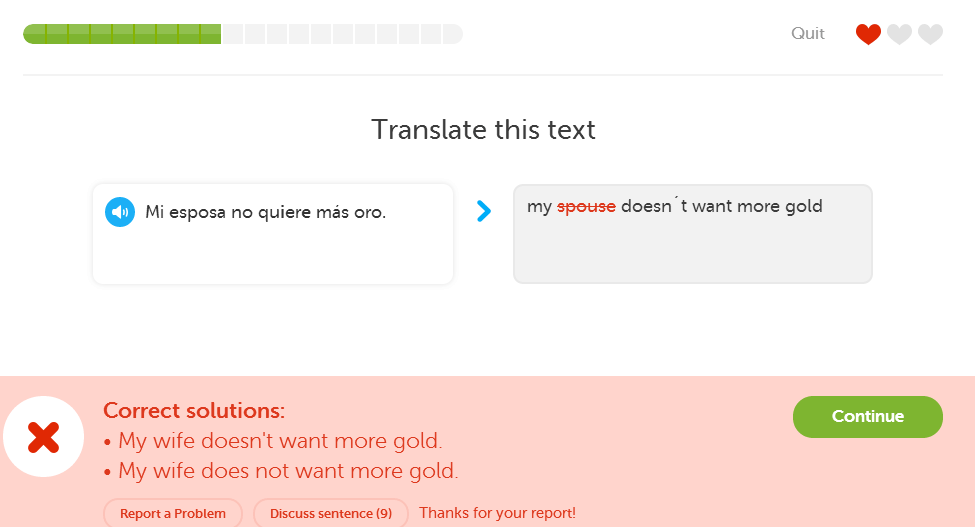
\includegraphics[width=0.7\textwidth]{Images/Theory/DuolingoPlacementTest.png}
    \centering
    \caption{Spanish placement test in Duolingo.}
    \label{fig:dulingo_placement_test}
\end{figure}

\subsubsection{Player Skills}
As mentioned above, the player’s skill level needs to match the difficulty level of the game. The player’s skills also need to increase during the game, at the same rate as the difficulty of challenges. If not, the game could quickly get too challenging or too easy. Rewarding players appropriately when completing specific tasks, with points or similar, is an essential part of this process.

Again, in Duolingo, players are matched with the appropriate skill level, and as the game progresses, both the player’s skills and the level of difficulty grows. The placement test, see Figure \ref{fig:dulingo_placement_test}, makes sure that players are met with an appropriate level of difficulty. Also, players have to put their knowledge to the test before they are allowed to ascend to the next level. This additional test mechanism makes sure that users are qualified for new levels and prevents players from being demotivated from challenges that are too demanding.

\subsubsection{Control}
Another central element of good game design is control. The players should feel a sense of control over their actions in the game and transfer their intentions to in-game behavior. Essential aspects of the game to achieve this are intuitive interfaces and easy-to-use input devices. Controlling the game should be intuitive and straightforward. In addition to this, players should not make errors that are disturbing to the gameplay. If they do, recovering from their mistakes should be supported. 

Racing games are, in general, examples of games that are intuitive to maneuver. Custom racing wheel controllers mimic the action of actually driving a car, as seen in Figure \ref{fig:racing_wheel_controller}. Recovering from errors that are disturbing for the gameplay, such as flipping the car or driving off a cliff, is also usually supported with a “reset” button.

\begin{figure}[H]
    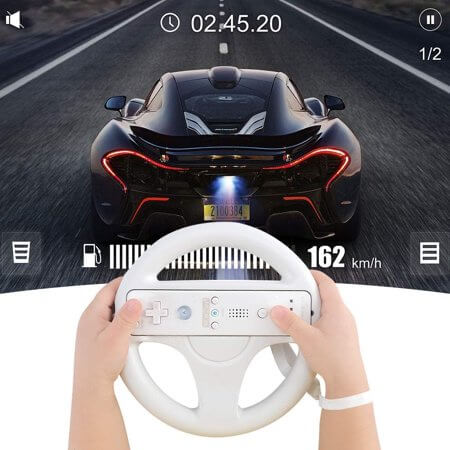
\includegraphics[width=0.5\textwidth]{Images/Theory/wii_racing_wheel_control.jpeg}
    \centering
    \caption{Wii Steering wheel used to play a racing game.}
    \label{fig:racing_wheel_controller}
\end{figure}

\subsubsection{Clear Goals}
Clear goals should be provided to the user at appropriate times. A primary goal should initially be presented to the user. Some introductory cinematic history that tells the story’s background is often used to describe this goal to the user. Intermediary goals should be provided to the user when they progress. Games often use “briefings” or “missions” for this. 

In Super Mario Bros, players are introduced to a mission of saving Princess Peach from the villain Bowser. This background establishes a clear goal for the entire game. The game also has intermediate objects of completing each level towards the final goal.

\subsubsection{Immersion}
Immersion describes a deep and effortless involvement in games. Players should feel engaged by the game to experience an altered sense of time, less awareness of surroundings, less self-awareness, and fewer worries. Immersion also indicates emotional attachment to the game. Examples of game elements that can increase immersion are audio and narratives. Sounds and music in games improve the players’ attraction to the game and keep them immersed for a more extended period. A history that gives the player some background information or a storyline also creates the same effect.

The role-playing game the Witcher 3 has become known for being a highly immersive open-world game. The game has a strong storyline, realistic graphics and audio, and many intermediate goals that draw the player deeper into the game, as seen in Figure \ref{fig:witcher3_immersion}. For Witcher 3, immersion can cause players to feel an emotional attachment to the game and reduced concern for self and sense of time.

\begin{figure}[H]
    \vspace*{0.5\baselineskip}
    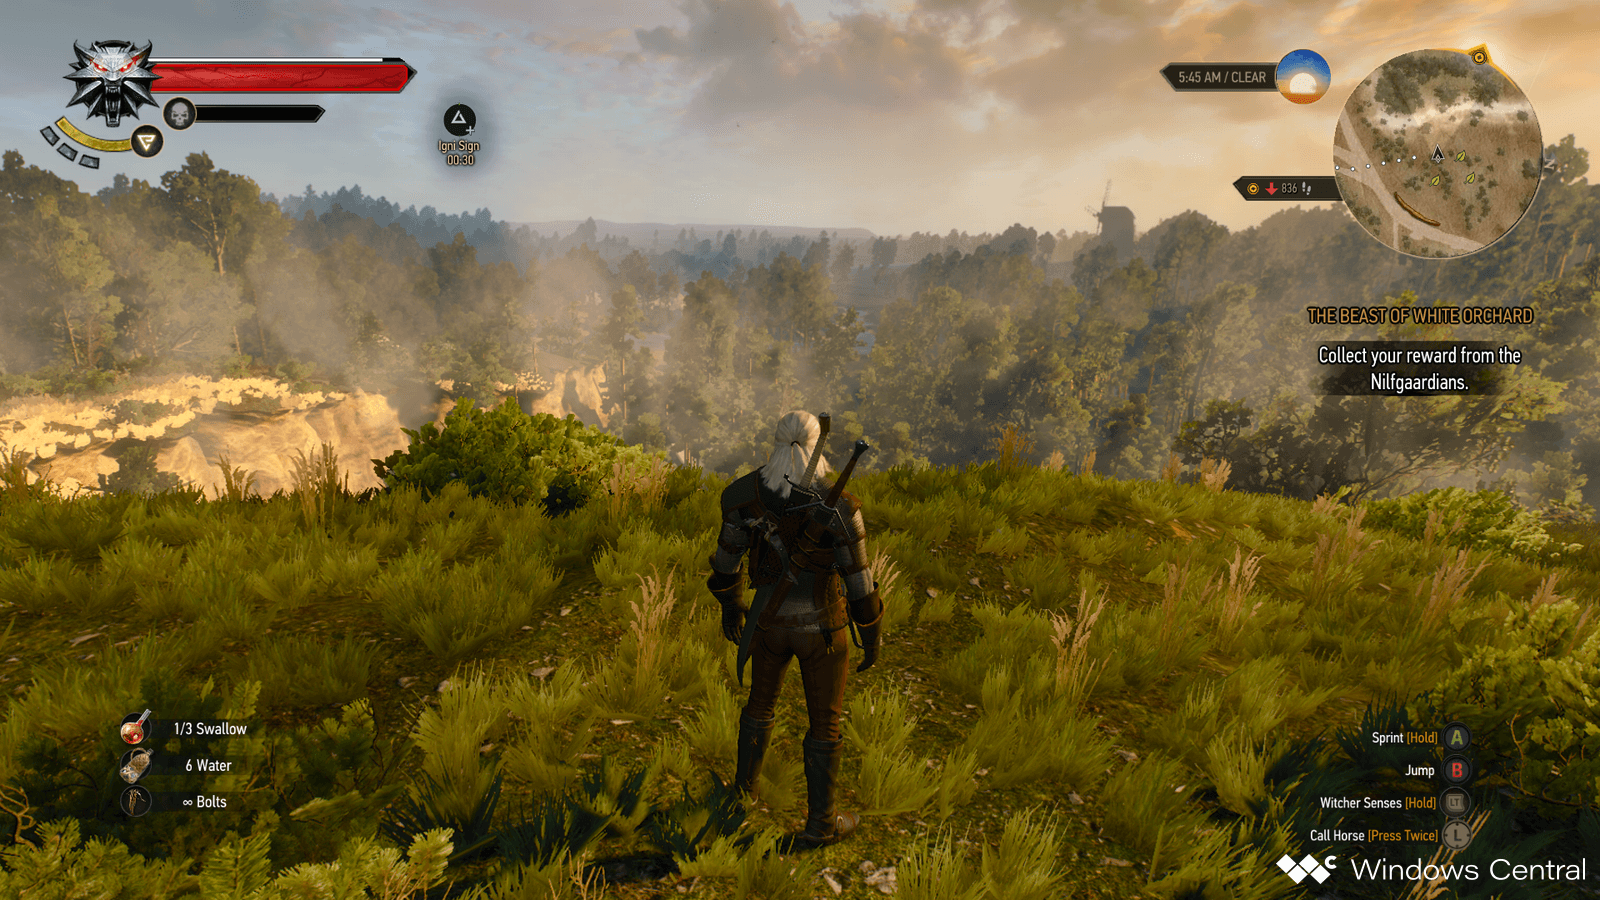
\includegraphics[width=0.8\textwidth]{Images/Theory/witcher3_immersion.png}
    \centering
    \caption{Screenshot from gameplay in Witcher 3.}
    \label{fig:witcher3_immersion}
    \vspace*{2\baselineskip}
\end{figure}

\subsubsection{Feedback}
\begin{wrapfigure}{r}{0.4\textwidth}
    \centering
    \vspace*{-1.5\baselineskip}
    
\includegraphics[width=0.3\textwidth]{Images/Theory/PokemonGoLevelUp.jpg}
    \caption{Feedback in Pokémon Go when leveling up.}
    \vspace*{-\baselineskip}
    \label{fig:pokemon_go_level_up}
\end{wrapfigure}
Players should get the feedback they need during the game. They should always know their status or score and progress towards the goal. Additionally, appropriate feedback based on their actions should be provided.

Pokémon Go uses direct and immediate feedback. Visual, textual, and audio feedback is used frequently. The game also uses points, levels, streaks, and medals to award good performance and engagement. Figure \ref{fig:pokemon_go_level_up} shows the visual feedback a player receives when leveling up in Pokémon Go.

\subsubsection{Social Interaction}
The last element in the GameFlow model is not an element of flow. Social interaction may often interrupt the immersion in games. However, it is an essential element in the GameFlow model because social interactions improve enjoyment in games. Games should support and create opportunities for player-to-player communication and social competitions. Online games are a typical example of how important social interaction can be. In this type of game, social interaction is often the main reason people are attracted to them. World of Warcraft is a classic example of such a game. 

Another example is social motives like affiliation and recognition in online fitness communities (OFC). A 2018 study on running motivations concluded OFC users are significantly more oriented towards achieving running goals and entering competitions than non-OFC users \citep{stragier_recreational_2018}. The results suggest that social gamification features such as recognition or leaderboards in these communities affect player motivation and enjoyment.

\subsection{Summary}
In this chapter, two frameworks describing how to create an enjoyable game have been presented. The frameworks include a description of central elements in game-design associated with producing good games. Even though all framework characteristics are essential aspects, a game should not necessarily incorporate all of them. As a game designer, the most valuable knowledge is understanding the theory and utilizing the appropriate parts.

The concept and elements proposed by \citeauthor{malone_what_1980} and \citeauthor{sweetser_gameflow_2005} will help invent new alternative games and develop our chosen concept later in this thesis. As described in the motivation (Chapter \ref{chap:motivation}), our focus is to create a socially beneficial alternative game. Consequently, the social element in the GameFlow model will be the essential consideration that should influence our game design. However, the other elements will also serve as guidelines and inspiration for us when developing the game. To what extent and which parts are used to create our game will be described later.

\clearpage

\section{Reward Systems}
\label{chap:reward_systems}

Reward systems play an essential role in every game. Players are motivated by rewards and reward systems to increase social meaning \citep{wang_game_2011}. Rewards are crucial for gamification applications where the concept often is built around introducing reward systems to enhance the users’ enjoyment.

\citeauthor{wang_game_2011} presents an article describing how reward systems are used in games and which design considerations a game developer should take into account. The paper proposes classifications for rewards, reward characteristics, and how players utilize them. In this chapter, the article’s key points will be presented, including the aspects just mentioned. After that, a summary of an article by \citeauthor{wang_effect_2016} illustrating the effect of game reward systems (points and audio) in Kahoot! will be given.

\subsection{Forms of Rewards}
Based on multiple studies done by other researchers, \citeauthor{wang_game_2011} proposed eight forms of rewards used in games to create positive experiences for the players:

\subsubsection{Score Systems}
Score systems are a type of reward that uses numbers to keep track of the player’s performance. Scores are considered crucial to the design of a fun game by many researchers and generally serve as a tool for self-assessment and comparison. The reward system is typically classified as a “glory” reward, i.e., it does not directly impact gameplay. World of Warcraft is an example of a game where the score system reward is used. The ladder system uses scores to determine player ratings. Figure \ref{fig:wow_player_rating} illustrates the game view showing the PvP rating in World of Warcraft: Battle for Azeroth.

\begin{figure}[H]
    \centering
    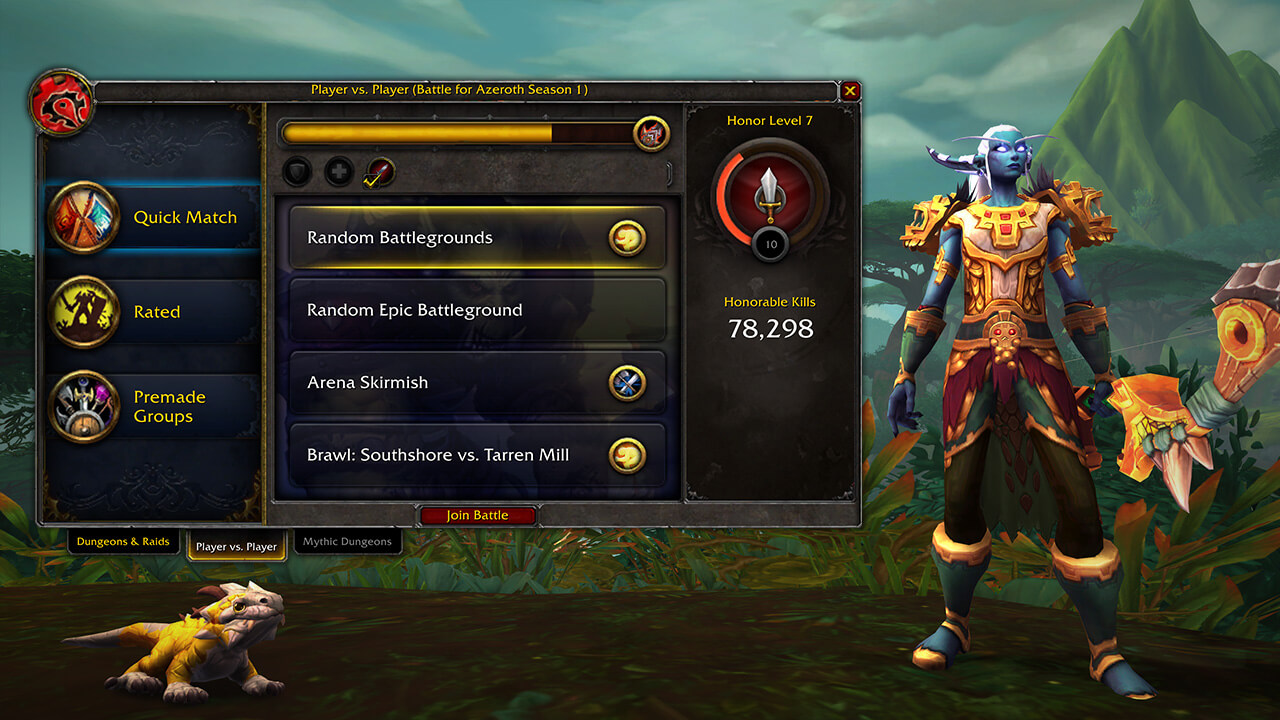
\includegraphics[width=0.75\textwidth]{Images/RewardSystems/WoWPvPRating.jpg}
    \caption{PvP player rating in World of Warcraft: Battle for Azeroth.}
    \label{fig:wow_player_rating}
\end{figure}

\subsubsection{Experience Point Reward Systems}
Experience Points (XP) are utilized in the majority of games where players control developable avatars. XP are typically used to measure the players’ progress in the game, leveling up when a certain number of points is reached. The reward is classified as a “facility” type of reward, meaning a reward that increases the avatar skills at certain levels. XP are similar to score systems described above but differ in at least three ways:
\begin{itemize}
    \item XP are bound to specific avatars rather than the player itself.
    \item XP are rarely used for a ranking purpose.
    \item XP directly affects gameplay.
\end{itemize}

\subsubsection{Item Granting System Rewards}
This type of reward consists of in-game items that players or avatars can use. Item granting systems are often adopted in RPGs and MMORPGs to encourage exploration of the game world. Their primary purpose is to maintain players’ interest in-between intense battles, missions, or other exciting moments. Figure \ref{fig:wow_player_rating} illustrates a typical avatar in World of Warcraft wearing rewarded items.

\subsubsection{Resources}
Resources are in-game valuables collected and used in a way that affects the gameplay. The reward system is similar to an item granting system. Still, there is a significant difference between the two: Resources are mostly for practical game use, while items have a collecting and social value only. An example of resources is virtual wood and stone in Age of Empires Online. Figure \ref{fig:resources_age_of_empire} illustrates the tribute part of the game where players can donate resources to other players.

\begin{figure}[H]
    \centering
    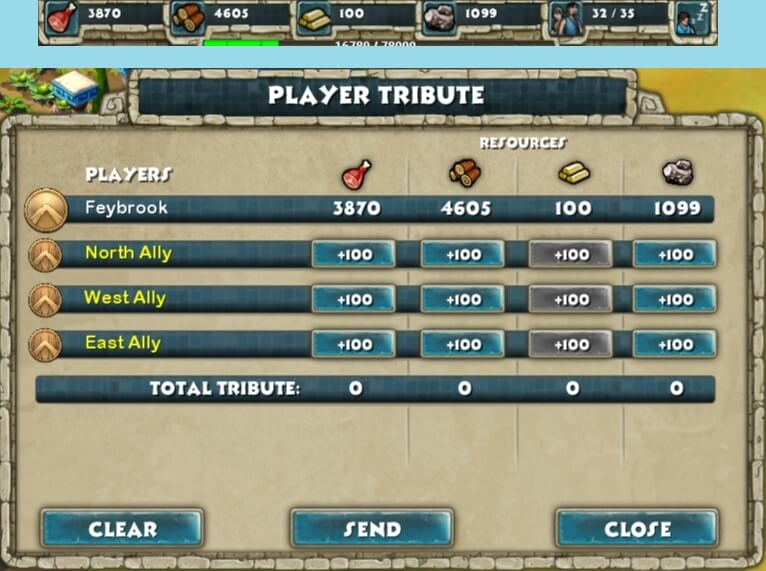
\includegraphics[width=0.75\textwidth]{Images/RewardSystems/AgeOfEmpireResources.jpg}
    \caption{Player tribute screen in Age of Empires Online.}
    \label{fig:resources_age_of_empire}
\end{figure}

\subsubsection{Achievement Systems}
Achievement systems consist of titles bound to a user or avatar collected by completing clearly stated requirements. This type of reward encourages players to complete certain tasks, which may be more challenging than what they otherwise would have considered doing. Achievements can also be a way of improving the players’ urge to explore the game world. As an example, there are over a thousand different titles in World of Warcraft. Collecting these is publicly acknowledged by the community, consequently encouraging players to complete these tasks. Figure \ref{fig:wow_achievements} illustrates the achievement screen in World of Warcraft: Legion.

\begin{figure}[H]
    \centering
    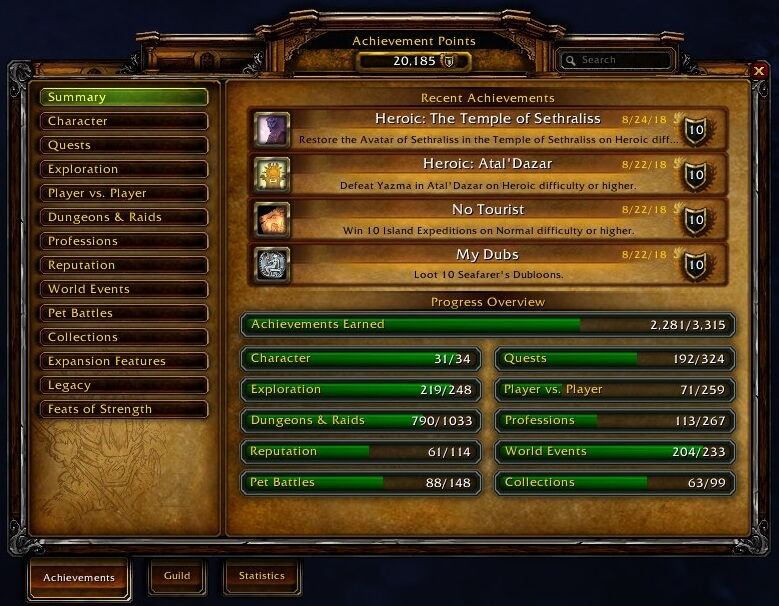
\includegraphics[width=0.75\textwidth]{Images/RewardSystems/WoWAchievements.jpg}
    \caption{Achievement screen from World of Warcraft: Legion.}
    \label{fig:wow_achievements}
\end{figure}

\subsubsection{Feedback Messages}
Feedback messages provide instant feedback, an important element of flow \citep{sweetser_gameflow_2005}, to the player. The reward is not collectible and thus cannot be used as a player comparison or directly affect the gameplay. In Dance Dance Revolution, a message with the word “Perfect” appears every time you perform the correct dance move with precise timing, as seen in Figure \ref{fig:dance_dance_revolution_perfect}. This game element is a perfect example of a feedback message reward. The feedback can also be pictures, sound effects, or video clips.

\begin{figure}[H]
    \centering
    
\includegraphics[width=0.75\textwidth]{Images/RewardSystems/DanceDanceRevolution.jpg}
    \caption{Screenshot from Dance Dance Revolution.}
    \label{fig:dance_dance_revolution_perfect}
\end{figure}

\subsubsection{Plot Animations and Pictures}
Plot animations or pictures are used in games following notable events, such as completing a level or a mission. The purpose of this reward is to motivate players to continue advancing in the game. A famous plot animation is found in Super Mario Bros after completing a level. Figure \ref{fig:plot_animation_super_mario} illustrates this scene in New Super Mario Bros. U Deluxe.

\begin{figure}[H]
    \centering
    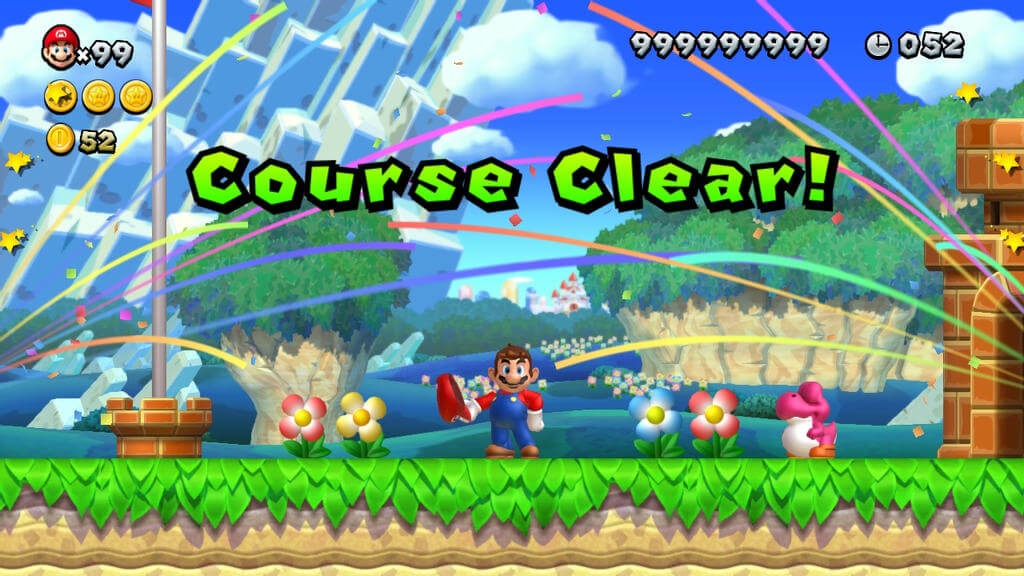
\includegraphics[width=0.75\textwidth]{Images/RewardSystems/SuperMarioBrosCourseClear.jpg}
    \caption{“Level completed” scene in New Super Mario Bros. U Deluxe.}
    \label{fig:plot_animation_super_mario}
\end{figure}

\subsubsection{Unlocking Mechanisms}
The last reward type is unlocking mechanisms, which give players access to new game content when certain conditions, such as a new level or a special environment, are met. Unlocking mechanisms are hiding elements and awarding them to players as they progress in the game. The reward is substantial in regards to maintaining player curiosity. An example is found in World of Warcraft, where avatars must achieve certain levels before accessing higher-level environments.

\subsection{Design Consideration}
The article proposes seven reward system design considerations, which are directly relevant for us when we are going to develop our alternative game concept:

\textbf{Life Constraint}\\
Rewards must be available in a manner that fits the intended target group of the game. Hardcore gamers tend to spend more time playing; thus, the rewards should take longer to obtain. However, if the game is designed for casual gamers, the rewards should be accessible during shorter sessions.

\textbf{Create Autotelic Experiences}\\
The rewards should create intrinsically rewarding experiences. One way of doing this is to develop multi-level goals which will keep their engagement in the game. Players will then also learn and experience the pleasure of learning. 

\textbf{Balance}\\
An essential part of designing reward systems is to balance the time spent with the value of the reward. It is frustrating for players to feel like the rewards are never valuable enough. On the other hand, if the rewards are too valuable, the player might appreciate them less. 

\textbf{Uncertainty and Secrecy}\\
Uncertainty in rewards can create additional fun in games, but appropriate handling is essential. Not all reward types are suited for secrecy. For example, ammunition and life counts are typical rewards that are preferred to be exposed to the player. Other kinds of rewards such as treasures and quests may be hidden to introduce more fun. Hiding these elements encourages players to dive deeper into the game and spend more time exploring it. 

\textbf{Accumulated vs. Instant Feedback}\\
Accumulated rewards are important attributes for marking progress and comparing status between players. Accumulated feedback is appropriate for creating long term and social sense of achievement. Contrary, instant feedback provides responsiveness and an element of flow to the game.

\textbf{Social Purposes}\\
Game rewards enable social status that can be shared with others. Hard to get rewards, such as special items, distinguishes advanced and casual players. These types of rewards also serve as a symbol to increase unity between skilled players.

\textbf{Physical World Activities}\\
Reward systems that support physical world activities impact the playing willingness. By being physically active, the guiltiness often associated with playing diminishes. An example is the physical world activities in Nintendo Wii, which changed the image of game playing.

\subsection{The Effect of Points and Audio in Kahoot!}
To conclude the topic of rewards systems in games, a concrete example of its importance will be briefly described. \citeauthor{wang_effect_2016} conducted a study in \citeyear{wang_effect_2016} looking at the effects of points and audio in the game-based learning system Kahoot!. Points as a reward system correspond to the “score systems” category, while audio classifies as “feedback messages,” according to the forms of rewards presented earlier in this chapter.  

The paper describes an experiment where Kahoot! was used as a learning method for teaching a lecture on software engineering. The students were divided into four groups using four different combinations of reward systems. The first group used Kahoot! as usual, with sound and audio. The second group played the game with audio but without points. The third group played Kahoot! without audio but with points, and the last group without audio and points. A questionnaire with statements related to concentration, engagement, enjoyment, learning, and motivation was filled out by the students after completing the lectures. 

The results from the study revealed notable differences in how the game was experienced in different groups. The effects of points and audio demonstrated a significant change in concentration, enjoyment, motivation, and engagement. The audio had a noticeable impact on classroom dynamics, but points also contributed to a more limited extent. An interesting observation was done in the group using Kahoot! where audio was removed, but points still present. The classroom was completely silent during the lecture, and students reported afterward that it felt more like a formal test than a game \citep{wang_effect_2016}.

The study illustrates the importance of reward systems in a game. Without points and audio in Kahoot! several of the students answered that they were less motivated and engaged.

\subsection{Summary}
In this chapter, a study of reward systems, including the eight different forms and seven design guidelines, has been introduced. In addition to this, a concrete example of the effects of reward systems in Kahoot! was presented. 

The content is highly relevant for our project and goal of developing an alternative game concept that has a socially beneficial effect. Especially in gamification concepts, reward systems are an essential tool for creating enjoyable games. In part \ref{part:hover}, where our concept is presented, a concrete description of how reward systems are used will be given.

\clearpage

\section{Player Types}
\label{chap:player_types}

Understanding player types and motivations are essential for designing games. This is because changes in game business practices have elevated the need for distinguishing player types and player styles, similar to how segmentation is used in marketing. Players can have very different interests in playing, which are important to consider when designing games. This chapter takes a look at \citet{hamari_player_2014} of player types. The article presents different approaches and understandings of player topologies found in previous literature. 

The use of segmentation has always been a central part of marketing practices. This practice implies that products are designed with specific end-users in mind as opposed to mass-marketing. The goal of segmentation is to identify homogeneous customers, to offer products that better match their needs. There are four categories of segmentation established in marketing theory; geographic, demographic, psychographic, and behavioral segmentation. \textit{Geographic} segmentation divides people into groups based on their geographical region. \textit{Demographic} segmentation divides people into groups based on descriptive features such as age, gender, occupation, and education. \textit{Psychographic} segmentation divides people based on personal traits, such as attitude, interests, lifestyle, and values. And, \textit{Behavioral} segmentation categorizes people into groups based on behavioral patterns observed in people.

Out of the four categories, geographic and demographic segmentation have not been of primary interest due to their irrelevance to game design. \citet{hamari_player_2014} explicitly states that their review attempts to conceptualize motivations, behavior, and traits that categorize within the psychographic and behavioral segments. The two segmentation categories are often challenging to distinguish, and \citet{hamari_player_2014} states that the literature interprets these differently. The game genres covered in \citet{hamari_player_2014} vary; however, Massive Multiplayer Online(MMO) games are more recurring than others.

\subsection{The Four Archetypes}
Though \citet{hamari_player_2014} review several papers on player topologies, many of them seem to stem from the core principles of Bartle’s four player types  (\citeyear{bartle_hearts_1996}). The player types, also known as Bartle’s taxonomy, are the result of observations Bartle made in player behavior in Multi-User Dungeons (MUDs). Through his observations, he created a two-dimensional model where each quadrant represents a player type, see Figure \ref{fig:bartle_playertypes}. The model’s two dimensions to playing are action vs. interaction, and player-orientation vs. world-orientation. Based on players’ position on the axes, one can distinguish players into the four player types; \textit{Achievers}, \textit{Explorers}, \textit{Killers}, and \textit{Socializers}. An Achiever is a player that prefers world-oriented actions to achieve measurable rewards like points. An Explorer is a player that prefers interaction in the game world, like discovering new areas. A Killer is a player that prefers action towards other players and thrives on competition. And a Socializer is a player that prefers interaction with other players over the game itself.

\begin{figure}[H]
    \centering
    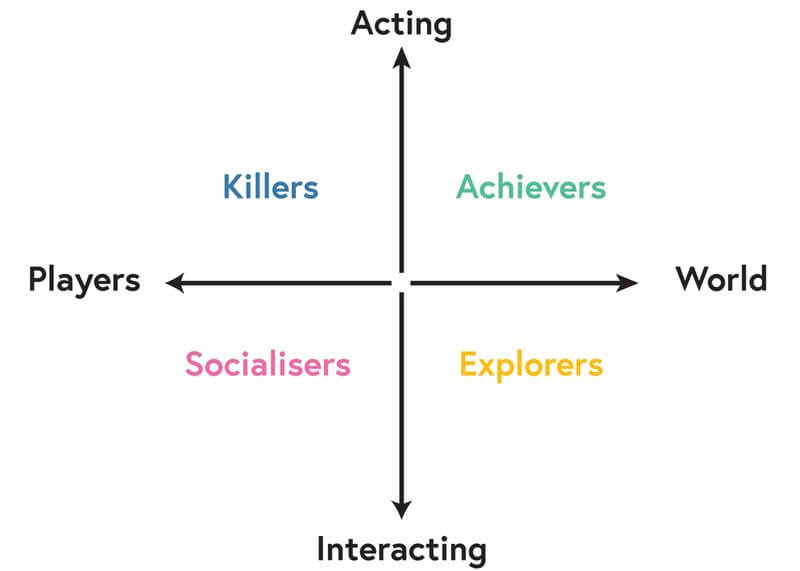
\includegraphics[width=0.75\textwidth]{Images/Theory/bartle_playertypes.jpeg}
    \caption{Bartle’s player types model \citep{bartle_hearts_1996}.}
    \label{fig:bartle_playertypes}
\end{figure}

Although Bartle’s model on player types is insightful, it has received criticism for being too generalizing. Besides, it does not consider that players can have multiple motivations or that their motivations for playing may change over time, making it difficult to pinpoint a player type. \citet{hamari_player_2014} emphasizes that the criticism stems from how the topologies have been used and suggests that the dimensions can be used as scales rather than nominal categories.

\citeauthor{hamari_player_2014} also review the work of \citet{yee_motivations_2007}. \citet{yee_motivations_2007} observes player motivations in MMORPGs, and builds on \citet{bartle_hearts_1996}, however \citeauthor{yee_motivations_2007} suggest that there are only three main motivational factors of motivation, with additional sub-factors. The main factors are Achievement, Social, and Immersion. Yee’s underlying facets of Achievement and Social have a resemblance to Bartle’s heuristics found in Achievers, Explorers, and Socializers; however, they are not perfectly comparable. Moreover, Bartle did not consider Immersion explicitly, while \citep{yee_motivations_2007} found that immersion was a major motivational factor for players.

\subsection{Hamari and Tuunanen’s Proposed dimensions}
The review on player topologies is extensive; however, it is surprisingly uniform. Hamari and Tuunanen suggest that the results can be summarized as seven dimensions, based on recurring ideas from the reviewed papers.

\textbf{Achievement}\\
\textit{Related keyword: Achiever, Single-oriented player, Guardian/Achiever, Aggressive gamer, Achievement, Progress \& provocation, Power \& domination, Runner, Hard fun, Casual, Avatar level, (Semi-)professional.}

The achievement dimension focuses on single world-oriented players that thrive on rewards, progress, provocation, and power. 
    
\textbf{Exploration}\\
\textit{Related keywords: Explorer, Solver, Rational/Explorer, Aggressive gamer, Social gamer, Immersion, Exploration \& Fantasy, Story \& escapism, Curiosity.}

The Exploration dimension is about exploring the game world. The player are driven by curiosity, fantasy, and storyline to escape the real world.
    
\textbf{Sociability}\\
\textit{Related keywords: Socialiser, Social mentalities, Community-oriented player, Idealist/Socialiser, Social, Helping \& support, the people factor, Friends \& Collaboration, (Semi-)professional, Amateur.}

The Sociability dimension is about community-oriented players who enjoy and are motivated by other players’ support and presence. 
    
\textbf{Domination}\\
\textit{Related keywords: Killer, Artisan/Killer, Aggressive gamer, Off-real world-oriented player, Progress \& provocation, Power \& domination, Casual.}

The domination dimension is about the player’s need for aggressive gameplay. This could be players trying to accumulate as much gear as possible or damage others, leading to the underlying desire of feeling powerful.

\textbf{Immersion}\\
\textit{Related keywords: Immersion, Committed mentalities, Exploration \& fantasy, Story \& escapism, Off-real world-oriented player, altered states, Hardcore.}

The Immersion dimension is about the degree to which players are committed and immersed in the game. Players may be driven by exploration, story, and fantasy. 
    
\textbf{Gaming intensity and skill}\\
\textit{Related keywords: Hardcore, Committed mentalities, Aggressive gamer, Veteran, Casual, Casual mentalities, Inactive gamer, Pacifist, Avatar level, Amateur.}

The Gaming Intensity and skill dimension are about the player’s commitment, experience, and attitude towards the game. Players are often said to be casual or hardcore players. Hardcore players are usually experienced and highly skilled, whereas casual players might be less experienced and less committed.  Players are placed by their willingness to participate, make an effort, and play.
    
\textbf{In-game demographics}\\
\textit{Related keywords: Avatar class and profession, non-clan member, Amateur, Professional, Group centrality, Size of the guild, Type of server, Faction.}

The In-game demographics dimension is about the player’s progress vs. their role. Examples of this can be different avatar classes, in-game professions, and positions in the hierarchy. For instance, players can pursue to level up their avatar from warrior to king as they progress in the game.

Though the papers are not directly comparable, because of their different scope, Hamari and Tuunanen go on to suggest that these seven recurring dimensions instead can be considered as five key dimensions and two supporting dimensions of player motivations. Achievement, Sociability, Exploration, Domination, and Immersion are the five key dimensions, and Game intensity and In-game demographics are the supporting dimensions. The reasoning behind this seems to be about the motivation of play. Achievement and Sociability seem to be the most recurring concepts in the literature; Immersion and Domination appear in some papers, whereas In-game demographics were only found in a few papers.

\subsection{Player Types and Reward Characteristics}
In the light of Hamari and Tuunanen’s player types, it is logical to see this in context with \citet{wang_game_2011} work on reward systems, previously discussed in \ref{chap:reward_systems}. \citet{wang_game_2011} review also presents four reward characteristics that can be used to analyze the influence of reward systems on different kinds of players.

The first one, social value, can be used for comparison of players or social interaction. This type of reward characteristic is particularly attractive for Socializers and Achievers. Rewards in games make it easier for players to compare themselves against others. An example is a high score list. The player can compare their points to others to see how they rank. Another good example is how hard-to-get items often draw attention. 

The next characteristic looks at “how rewards affect gameplay”. For this particular characteristic, it is interesting to see how rewards can help the player advance in the game, motivate them to produce new content, and participate in the game. Using the player types from Bartle’s taxonomy, \citet{wang_game_2011} summarizes the effect reward has on different player types as:

\begin{itemize}
    \item \textbf{Achievers and Killer:} Most interested in accumulating rewards that are evidence of their advanced skills and do not care about the visual aspect.
    \item \textbf{Socializers:} Greater interest in rewards that can draw attention to them, e.g., hard to get items.
    \item \textbf{Explorers:} Like Achievers and Killers, the motivation behind is gaining sufficient strength to explore game world details.
\end{itemize}

The third attribute is “suitability for collection and review” \cite{wang_game_2011}. The logic behind this is that building a sense of accomplishment improves the ability to preserve game memories. Collecting rewards is also a tool for players to recognize other players with similar interests. An important design consideration for this attribute is to showcase the rewards, so they are easy to present and review in the game. For instance, medals or badges that indicate game status or ranking can be showcased on the player’s profile. The rewards could then strengthen the sense of collection and produce a feeling of completion and perfection among the players.
The last characteristic is “the time required to earn and/or receive a reward“ \cite{wang_game_2011}. In contrast to real-world rewards, e.g., job promotion, a game reward can be instantaneous or rewarded after a couple of hours of gaming. A player may, for example, get a new level as a reward after a couple of hours of play. The time and intensity required to earn a reward are crucial aspects of game design that must be carefully planned to create a positive player experience.

Though most of the player topologies have been built on observations of MUDs, MMORPGs, and other online games, the topologies seem to be relevant for various game types. The results can, for instance, be applied in the context of gamification, where game mechanics related to sociability and achievements are frequently used. Some of these mechanics can be social rewards such as likes and comments or achieving good results, and breaking records for other players to see.

\subsection{Summary}
This chapter has introduced different interpretations of player types. We looked at the recurring ideas present in literature and have concretized them into seven primary dimensions. Depending on the game concept and genre, game designers may use Hamari and Tuunanen’s dimensions to create organic game environments that offer rewarding gameplay for different player types. The dimensions and understandings from this chapter will be useful later for developing new game concepts and for the design, development, and analysis of the final game.
\clearpage

\section{What is an Alternative Game?}
\label{chap:what_is_alternative_game}

To develop a concept for an alternative game, a clear understanding of which games can be categorized as alternative games are crucial. Let us first take a look at what the word “alternative” means in this context with some definitions from three well-known dictionaries:

\blockquote{
    \textit{“Different from the usual or traditional way in which something is done”} \\
    \textbf{Oxford learner's dictionary}
    
    \textit{“Different from the usual or conventional”} \\
    \textbf{Merriam-Webster's Collegiate Dictionary}
     
    \textit{“Alternative things are considered to be unusual and often have a small but enthusiastic group of people who support them”} \\
    \textbf{Cambridge dictionary}
}

While all of these dictionaries define the word differently, we can see that there are some commonalities. All three describe alternative as something “unusual” or “different from the usual.” The key takeaway from the definitions is that an alternative game is a game where the creators have done something to differentiate the game from ordinary ones.

To increase the ability to recognize alternative game concepts more efficiently, we will examine existing alternative games and analyze their commonalities. The research result is a list of six characteristics where alternative games often differ from regular games. The characteristics can be illustrated in a model which helps recognize and invent alternative games.

\subsection{Alternative Game Characteristics}
Our proposal of what alternative games are is then the following:

\textit{If a game deviates from regular games in one or more of the game characteristics categories, \textbf{input}, \textbf{output}, \textbf{target group}, \textbf{game genre}, \textbf{domain}, \textbf{interaction}, or \textbf{model}, it can be considered an alternative game.}

The six characteristics are based on recurring observations found in different game concepts. Below are explanations of all categories with coherent, relevant alternative games presented. These categories are covering all alternative games we have studied during this phase of the project. However, it is important to point out that additional characteristics from games that are not developed yet, or we are not aware of, might exist. As technology moves forward, it is reasonable to assume that new branches of alternative games might emerge.

\subsubsection{Input}
A common way of creating an alternative game is to use an unusual input source (such as the GPS, microphone, special controllers, or accelerometer) for controlling the game. Using input sources such as GPS has become more regular in recent years, although it is still not mainstream. Three examples of games using alternative input sources are Knowledge War \citep{wang_knowledge_2016}, CityZombie \citep{zhu_experiences_2010} and Exermon \citep{wang_evaluation_2017}. Both Knowledge War and CityZombie use the user’s position as a central part of playing the game. Moving around in the real world translates to the gameplay. Exermon is an example of utilizing the accelerometer on the player's phone. The game is a strength-based exercise game that tries to motivate people to do more strength exercises. An alternative input source, the accelerometer, is used to register the number of repetitions the user completes in one workout. 

\subsubsection{Output}
The output from the game is another characteristic commonly explored in the development of alternative games. Some known examples are sound, haptics, and augmented reality, but there are many more. Two examples of games using alternative outputs are “Unexceptional.net” and “The Amazing City Game.” Unexceptional.net is a story-driven pervasive game where “the story evolves through multiple media channels interacting with the player.” The game includes different untraditional outputs, such as SMS and phone calls, to provide feedback to the player \citep{wang_unexceptionalnet_2009}. The Amazing City Game is also a pervasive game where the players can play a knowledge competition tour. The game utilizes location and augmented reality to show different vital landmarks at a user’s location \citep{wang_pervasive_2011}. The number of location-dependent games and augmented reality games has, in recent years, increased. However, the technologies have yet to become common. 

\subsubsection{Target Group}
The target group is an essential characteristic of a game, and it decides what type of users the game should appeal to. Some games include adjustments to target specific groups of people, and some of these can make the game fall into the alternative game definition. More special target groups, like people with physical disabilities, often require more adjustments to play games at all. For example, people who cannot maneuver a game using traditional handheld controllers need other ways to interact. A Brain-Computer Interface (BCI) could be a way of bringing games to this group of people. One concrete example is the use of brain waves (via a \href{www.neurosky.com}{NeuroSky} brain set) to control the movement in a Snake game \citep{wang_using_2012}.

\subsubsection{Game Genre}
Computer games are generally categorized as one of eight game genres \citep{prensky_fun_2001}:

\begin{enumerate}
    \item Action Games
    \item Adventure Games
    \item Fighting Games
    \item Puzzle Games
    \item Role-Playing Games (RPG)
    \item Simulation Games
    \item Sports Games
    \item Strategy Games
\end{enumerate}

Earlier computer games were usually limited to one category, while today, games often fall into multiple ones. Additional categories may also be defined for games that do not directly belong to any of these genres. Alternative games usually consist of unique concepts and uncommon gameplay, often falling into other categories than those mentioned above. An example of such a genre is gamification, defined as “the application of game design principles in non-gaming contexts” \cite{robson_is_2015}. An example of a game not fitting directly into any of the eight general game genre categories but utilizes gamification is the “Kinect Recycling Game.” This game is a gamification concept of recycling trash, where the goal is to teach recycling in an engaging and realistic manner. As the name implies, the game uses Kinect to recognize players' hand gestures to place the trash into the correct bins \citep{wang_learning_2015}.

\subsubsection{Domain}
Computer games can be applied to different domains. The domain of a game depends on what area of use it serves. Some examples of game domains are entertainment, education, industry, government, and health. Alternative games may sometimes define their area of use, where the new domain may be a combination of other domains or a subset of an existing domain. For instance, edutainment games are a crossing between education and entertainment. Another example of an alternative domain is Attensi’s system for gamified work training, mixing industry, and learning \citep{attensi_why_2020}. The company offers tailored 3D job simulators to large organizations to achieve tangible and measurable changes in employees’ behavior and skill

\subsubsection{Interaction}
There exist a lot of various interaction forms for games. Examples included cooperation, competition, player vs. player (PVP), and more. Interaction can also contain an alternative twist, i.e., interaction forms that are not used in ordinary games. One such concept is the multimodal “Multiplayer On One Screen Entertainment System (MOOSES)” approach. Here, many players use their smartphones as controllers for gaming on a shared screen \citep{wang_evaluation_2010}. \href{http://www.airconsole.com}{AirConsole} is a concrete example of where this concept is utilized. The console includes multiple MOOSES based games where the players use their smartphones as controllers. Games can also be pervasive, meaning the game experience is extended beyond the fictive world. The player interacts with both the virtual and real worlds.

\subsection{Model}
Based on these six characteristics, we have created a model to help us compare alternative game concepts, see Appendix \ref{appendix:complete_model}. The model categorizes a game’s properties using the six categories to compare and justify why concepts can be described as alternative games. Thus, the model will help describe existing alternative games in Chapter \ref{chap:existing_games} and new ideas in Chapter \ref{chap:new_ideas}.

Additionally, the model is useful for inventing new alternative game concepts by exploring the characteristics separately. Modifying properties in each characteristic one by one can create ideas that would otherwise not have come up. It will also improve the structure of an idea brainstorming session. Consequently, we will use the model in the brainstorming part of inventing new alternative games in Chapter \ref{chap:new_ideas}.

\subsection{Summary}
This chapter presented our definition of alternative games together with the six coherent categories of game characteristics. A short description of each of them with relevant examples from the literature was given. The chapter provides a more concrete understanding of an alternative game and a model to distinguish different concepts. This knowledge will help us later when we are going to invent and develop our alternative concept. In the next chapter, existing popular and known alternative games will be described. How they fit into the proposed categories in this chapter will also be outlined.
\clearpage

\section{Existing Alternative Games}
\label{chap:existing_games}

In this chapter, seven different alternative games will be presented. The games are picked based on popularity, relevance today, and how they compare to each other. Different types of games are carefully chosen to illustrate the diversity of alternative games that exist. A brief explanation of the game concept and why it is an alternative game will be given for each game.

\subsection{Hold}
Hold is an application that rewards players for not using their phones \citep{hold_hold_2020}. The game was initially launched in 2016 for iOS and Android, focusing on Norwegian university students \citep{ringheim_smarttelefon_2018}. Since then, the application’s target group has expanded beyond this focus. 

\begin{figure}[H]
    \begin{minipage}{.5\textwidth}
      \centering
      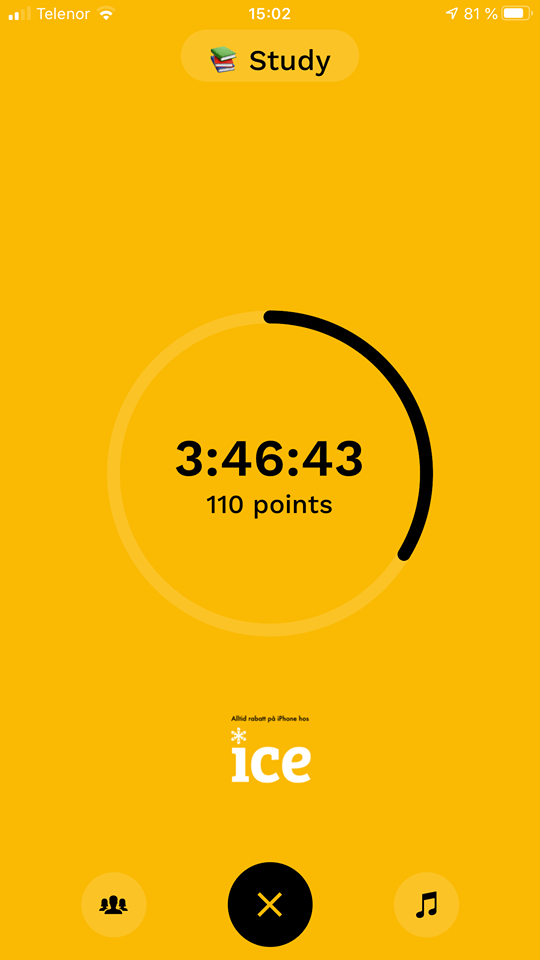
\includegraphics[width=.75\textwidth]{Images/ExistingGames/HoldApp.png}
      \captionof{figure}{Main timer screen in Hold.}
      \label{fig:hold_timer}
    \end{minipage}
    \begin{minipage}{.5\textwidth}
      \centering
      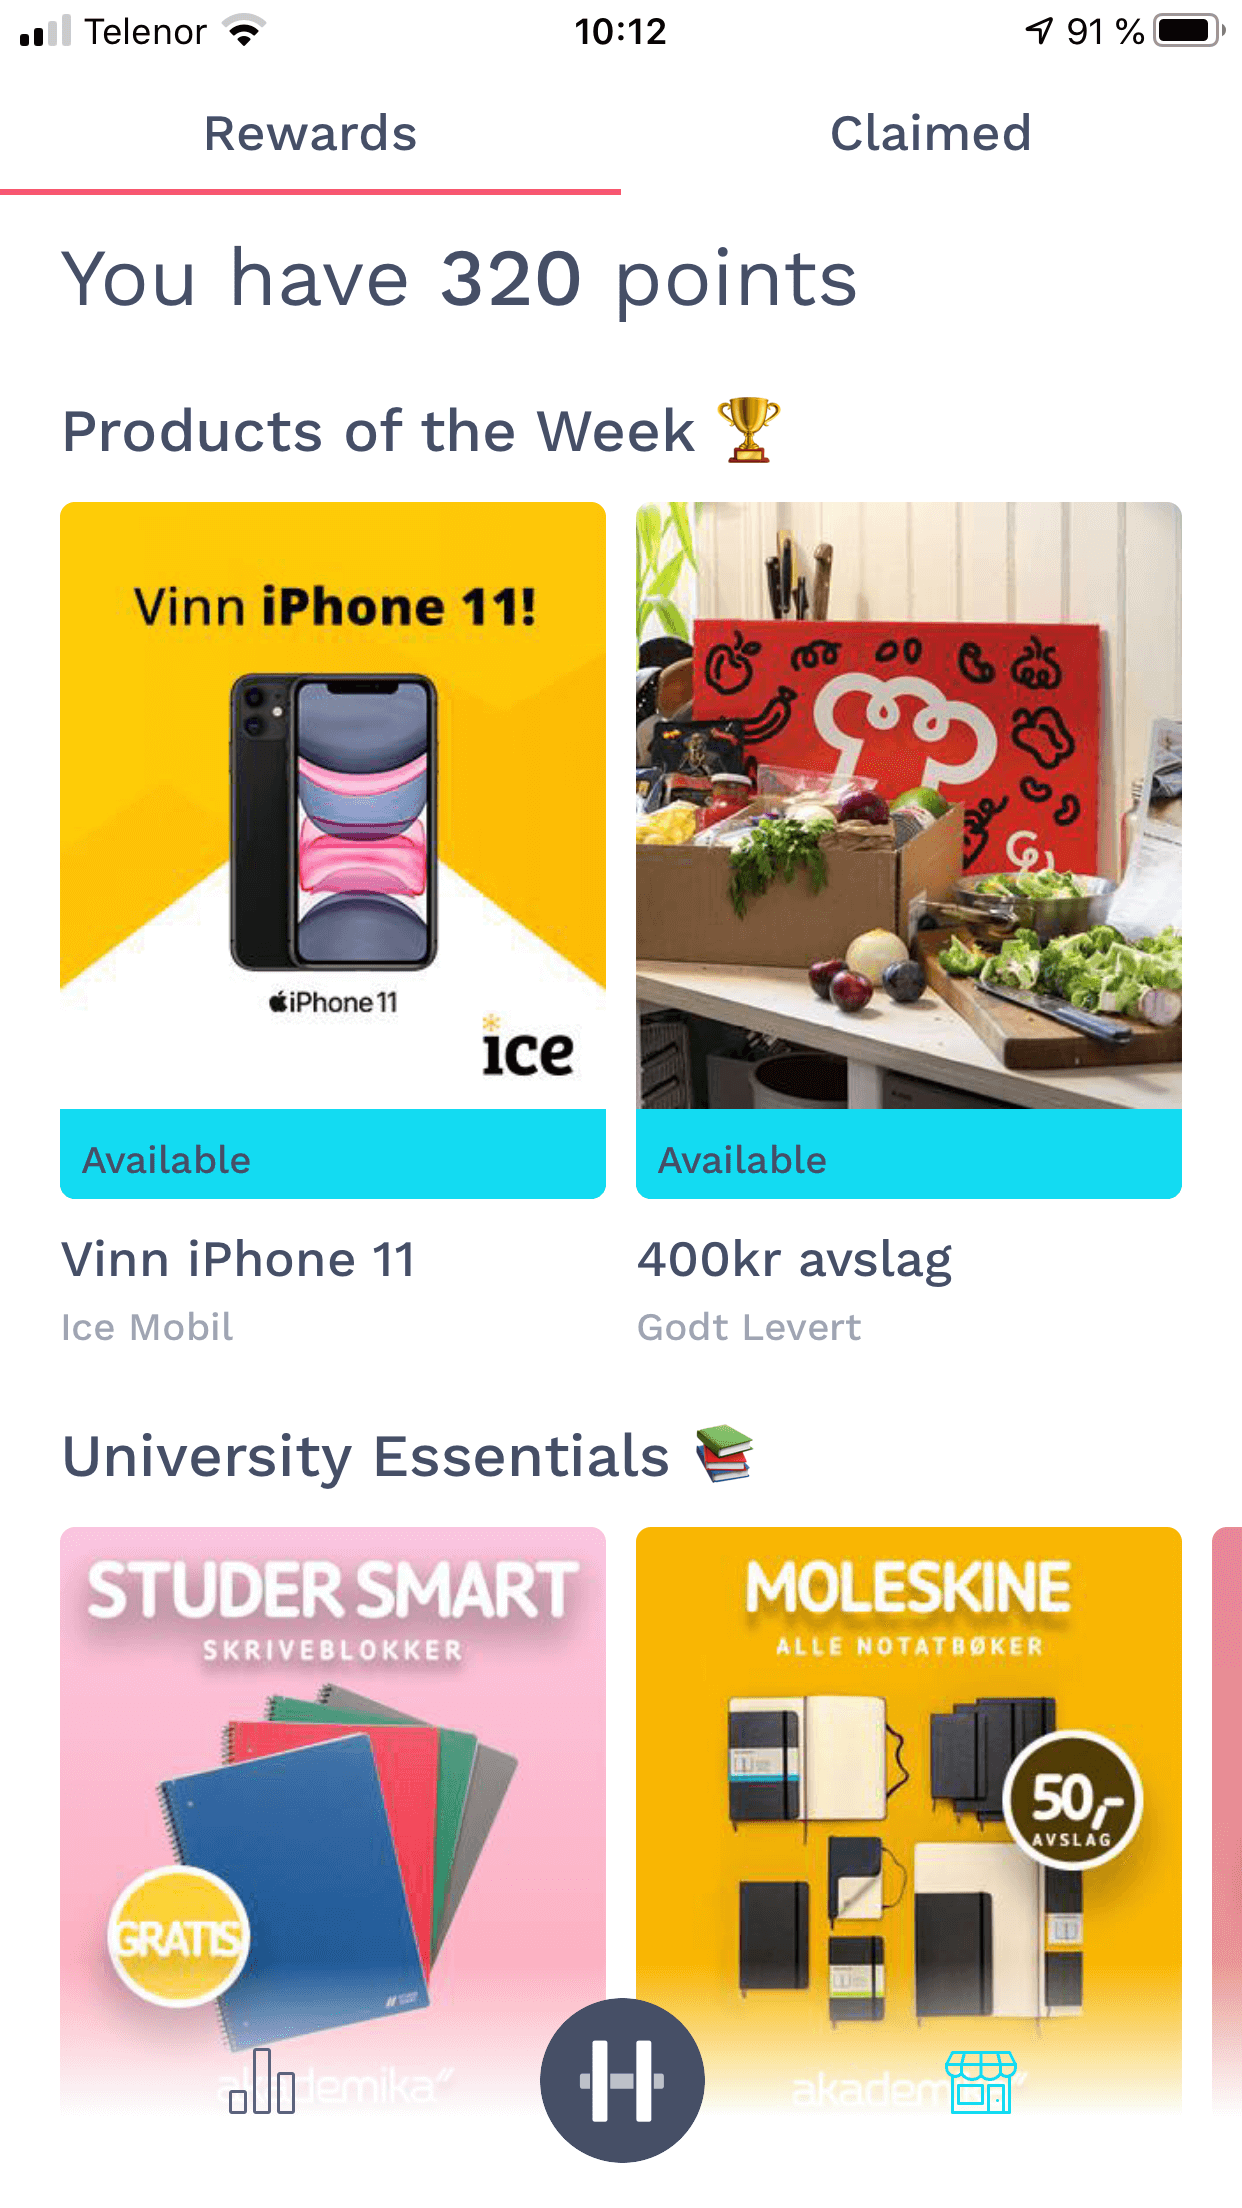
\includegraphics[width=.75\textwidth]{Images/ExistingGames/HoldAppRewards.png}
      \captionof{figure}{Choices of rewards in Hold.}
      \label{fig:hold_reward}
    \end{minipage}
\end{figure}

The application helps players limit distractions through gamification. When a player activates the application, a timer starts running (see Figure \ref{fig:hold_timer}). The player is rewarded ten points for each twentieth minute they are not using their phone. The points can later be exchanged into real-life items such as coffee, food, or discounts, as seen in Figure \ref{fig:hold_reward}. The rewards are the primary motivating factor for using the application.

Unlike other games, Hold’s concept is to encourage people not to use their mobile phones. The player can choose to play alone against the environment (PvE) or connect with friends to compare scores, making it more competitive (PvP). The application also lets players connect with nearby friends through Bluetooth, enabling them to focus (collaborate) while boosting their points collectively \citep{wakefield_free_2018}.

Hold is a perfect example of an alternative game with a different concept, where the developers have explored multiple of the game characteristics categories. The game classifies as alternative primarily for two reasons: It explores alternative game genres by using gamification, rewarding the player points for not using their phone. Furthermore, it uses an alternative input source, Bluetooth, for connecting with nearby friends.

\subsection{Mario Kart Live: Home Circuit}

\begin{figure}[H]
    \centering
    
\includegraphics[width=0.8\textwidth]{Images/ExistingGames/MarioKartLive.jpeg}
    \caption{Mario Kart Live poster illustrating gameplay.}
    \label{fig:mario_kart_live}
\end{figure}
Mario Kart Live is a newly developed augmented reality (AR) concept from Nintendo (released 16th October 2020) for its Switch game console. The game is based on the classic Mario Kart game, but with a unique twist: the inclusion of a specially designed racing kart that follows the player’s maneuvers in-game. A live video feed from the racing kart is relayed to the player’s Switch, mapping the virtual track to the player’s home \citep{velazco_race_2020}. The game can be played individually (against AIs) or as a multiplayer game with more than one kart \citep{hashimoto_mario_2020}.

The game is a typical example of how alternative sources for input and output can bring something new to an already familiar game concept. For this Mario Kart game, the alternative twist is to use a camera to produce AR output. Figure \ref{fig:mario_kart_live} shows a poster from the game where you can see the karts racing a player’s home and how the game is presented to the player. 

\subsection{Pokémon Go}
Pokémon Go is another good alternative game example, published and developed by Niantic for iOS and Android. The game was launched in 2016 and quickly became one of the most popular mobile games of all time \citep{grubb_pokemon_2016}. The concept is an extension of the classic Pokémon game found on multiple of Nintendo's handheld devices.

\begin{figure}[H]
    \begin{minipage}{.475\textwidth}
      \centering
      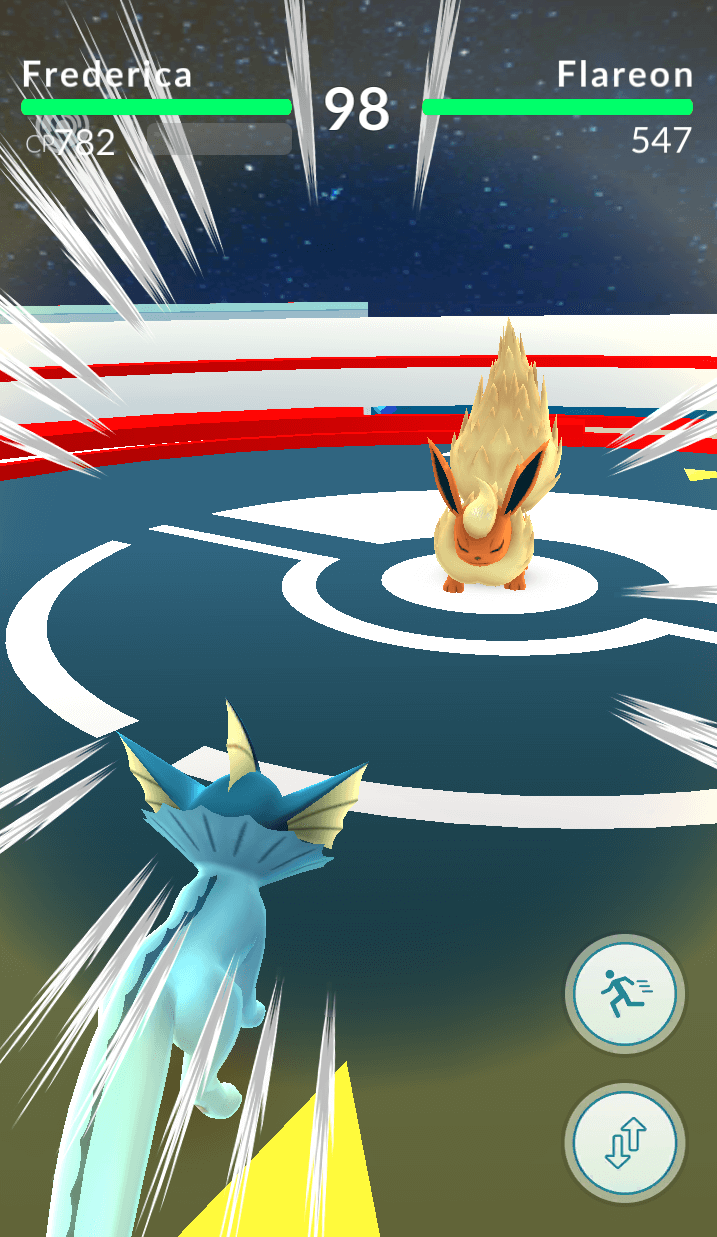
\includegraphics[width=.8\textwidth]{Images/ExistingGames/PokemonGoBattle.png}
      \captionof{figure}{Screenshot of an ongoing battle in Pokémon Go.}
      \label{fig:pokemon_go_battle}
    \end{minipage}
    \hspace{0.5cm}
    \begin{minipage}{.475\textwidth}
      \centering
      
\includegraphics[width=.7\textwidth]{Images/ExistingGames/PokemonGoCatch.png}
      \captionof{figure}{Typical screenshot of gameplay in Pokémon Go.}
      \label{fig:pokemon_go_catch}
    \end{minipage}
\end{figure}

The concept is similar to the previous Pokémon games but utilizes AR and location determination (GPS) to find and catch Pokémons. The player needs to move around in the real world to play the game. Battles between Pokémons (to increase combat points and get prices) can happen at specific places known as Pokémon Gyms. These spots correspond to real-world points of interest (POI) such as parks and tourist attractions \citep{bastow_pokestops_2016}. There are also additional important POI in the game, such as PokéStops and Nests. Figure \ref{fig:pokemon_go_battle} is an in-game screenshot where you can see a typical Pokémon battle, while Figure \ref{fig:pokemon_go_catch} shows a screenshot of gameplay while catching a Pokémon.

The game is an alternative game as it explores uncommon input and output sources such as camera, GPS, and AR. The game is also classified as a pervasive game because the player experience is extended to the real world. A study on \textit{The Pikachu Effect} reveals that the magnitude of Pokémon Go players experience both physical and social benefits from the pervasive game\citep{kaczmarek_pikachu_2017}. Pokémon Go is an excellent example of how alternative games can become very successful.

\subsection{Just Dance Now}
Just Dance Now is an alternative game produced by Ubisoft, launched in 2014 \citep{fandom_just_2020}. The game is an addition to the Just Dance franchise, where the concept is to pick a song from the catalog and follow the moves of the on-screen character, see Figure \ref{fig:just_dance_now_pc}. 

\begin{figure}[H]
    \begin{minipage}[t]{.625\textwidth}
        \centering
        
\includegraphics[width=\textwidth]{Images/ExistingGames/JustDanceNow_Pc.png}
        \caption{Just Dance Now screenshot from a computer display.}
        \label{fig:just_dance_now_pc}
    \end{minipage}
    \hspace{.05\textwidth}
    \begin{minipage}[t]{.325\textwidth}
        \centering
        
\includegraphics[width=0.8\textwidth]{Images/ExistingGames/JustDanceNow_Mobile.png}
        \caption{Just Dance Now screenshot from a smartphone.}
        \label{fig:just_dance_now_mobile}
    \end{minipage}
    \vspace*{\baselineskip}
\end{figure}

Just Dance Now distinguishes itself from the other games of this type by being more available because it does not require a dedicated gaming console. It can be played using an iOS or Android-based smartphone as the controller and a large screen connected to the internet, such as AppleTV, Chromecast, or a computer \citep{ubisoft_general_2020}. The player's smartphone is used as a movement tracker, and the large screen displays the dance moves they should perform. Multiple players can join the same game and dance together, competing to get the highest score.

This game can be viewed as an alternative game because of the use of the player’s mobile phone as a movement tracking device, as seen in Figure \ref{fig:just_dance_now_mobile}. Based on the sensors’ measurements in the player’s phone, the game determines whether or not the player is doing the dance moves well.

The interaction form is another reason why this game is an alternative game. The game is an example of a multi-modal exergame, where all players in one game use the same large screen to see the moves they need to perform in order to earn points. A recent study on the use of exergames in physical education in primary schools revealed that Just Dance Now had positive effects on students’ performance, engagement, and motivation for physical activity\citep{quintas_psychological_2020}. This concept can also be described as a “Multiplayer On One Screen Entertainment System” (MOOSES), presented in Chapter \ref{chap:what_is_alternative_game}. 

\subsection{Guitar Hero}
Guitar Hero is a series of games initially developed for PlayStation 2 in 2005. The game series later expanded to multiple other game platforms, including Xbox 360 and Nintendo Wii. The game concept is based on simulation and gamification of playing guitar, using a custom-developed guitar controller (see Figure \ref{fig:guitar_hero_controller}). The player tries to match the in-game “notes” with buttons on the guitar controller, resulting in a score coherent with the number of notes hit. Songs available to choose from vary between different games, but generally, they belong to the genre of rock \cite{metacritic_guitar_2020}. Figure \ref{fig:guitar_hero_screenshot} shows a screenshot example from playing the game in single-player mode. 

One of the categories of alternative game characteristics is input. As per the definition (in Chapter \ref{chap:what_is_alternative_game}), a game using alternative input sources can be classified as an alternative game. Guitar Hero is a typical example of such a game because it depends on a custom-designed controller for playing. Additionally, the use of gamification as the game genre is another reason why Guitar Hero can be defined as an alternative game. The central concept of the game can be perceived as gamification of playing guitar.

\begin{figure}[H]
    \begin{minipage}{.34\textwidth}
        \centering
        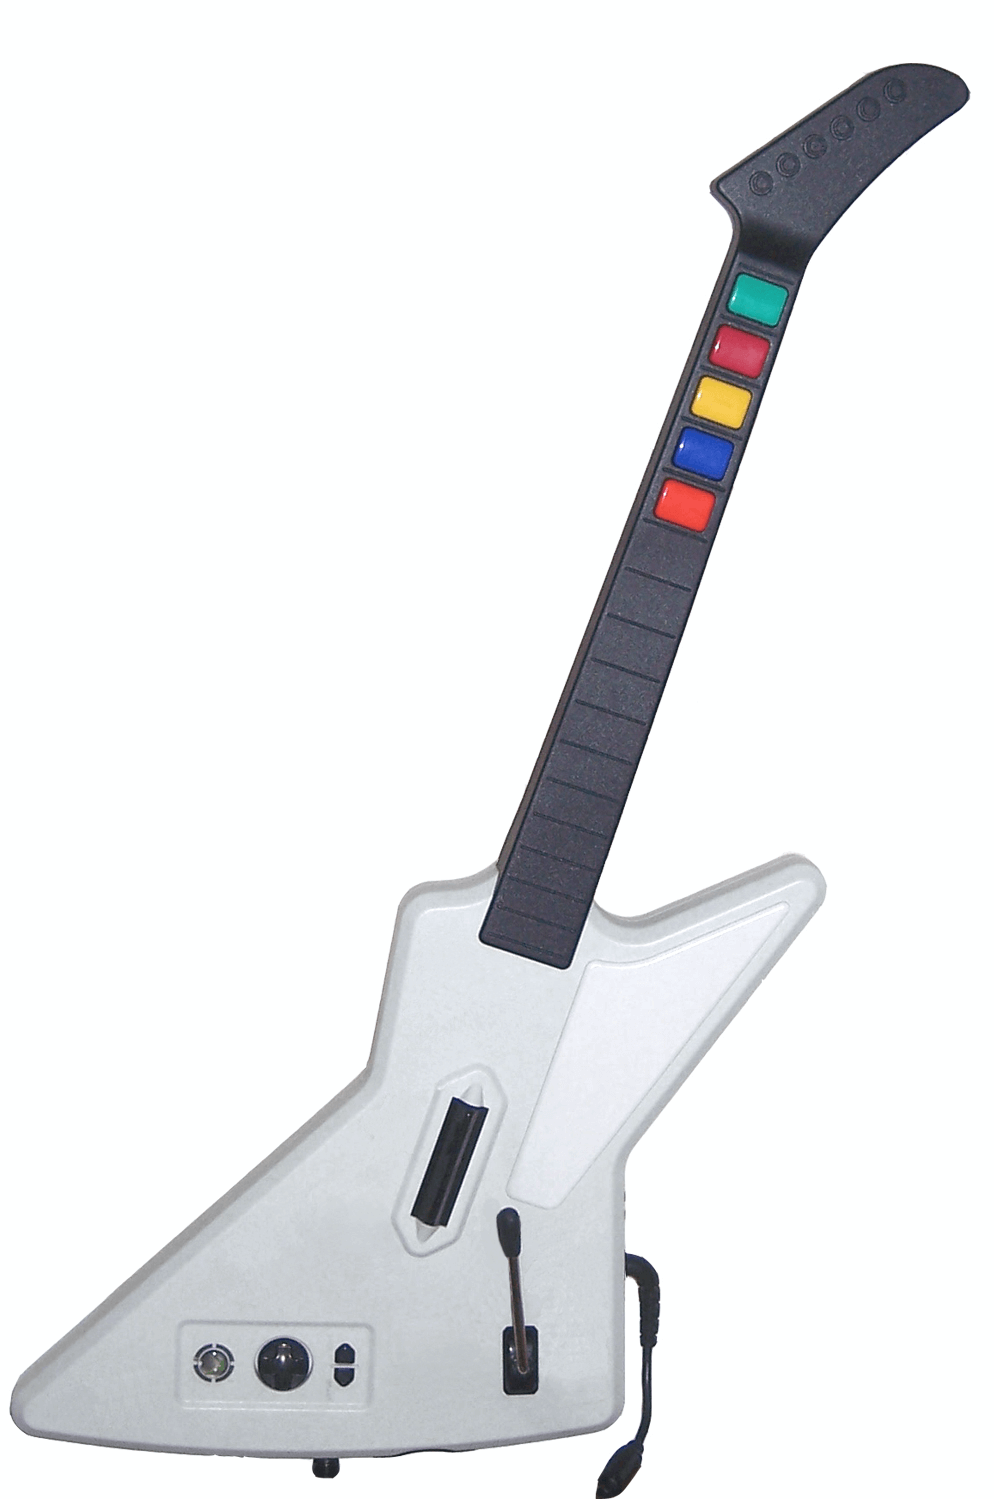
\includegraphics[width=0.9\textwidth]{Images/ExistingGames/GuitarHeroController.png}
        \caption{A Guitar Hero controller.}
        \label{fig:guitar_hero_controller}
    \end{minipage}
    \hspace{0.5cm}
    \begin{minipage}{.64\textwidth}
        \centering
        
\includegraphics[width=0.9\textwidth]{Images/ExistingGames/GuitarHeroScreenshot.jpg}
        \caption{Screenshot from gameplay in Guitar Hero.}
        \label{fig:guitar_hero_screenshot}
    \end{minipage}
\end{figure}

\subsection{Wii Fit}
Wii Fit is an exercise game (exergame) created and launched by Nintendo in 2007 \citep{imdb_wii_2020}. The game is only available on Nintendo Wii and requires a unique controller in addition to the regular Wii controller. Wii Fit is a collection of minigames that combine the two domains of health and entertainment. The game has four main exercise categories to choose from; strength training, aerobics, yoga, and balance \citep{ign_wii_2008}.

\begin{figure}[H]
    \centering
    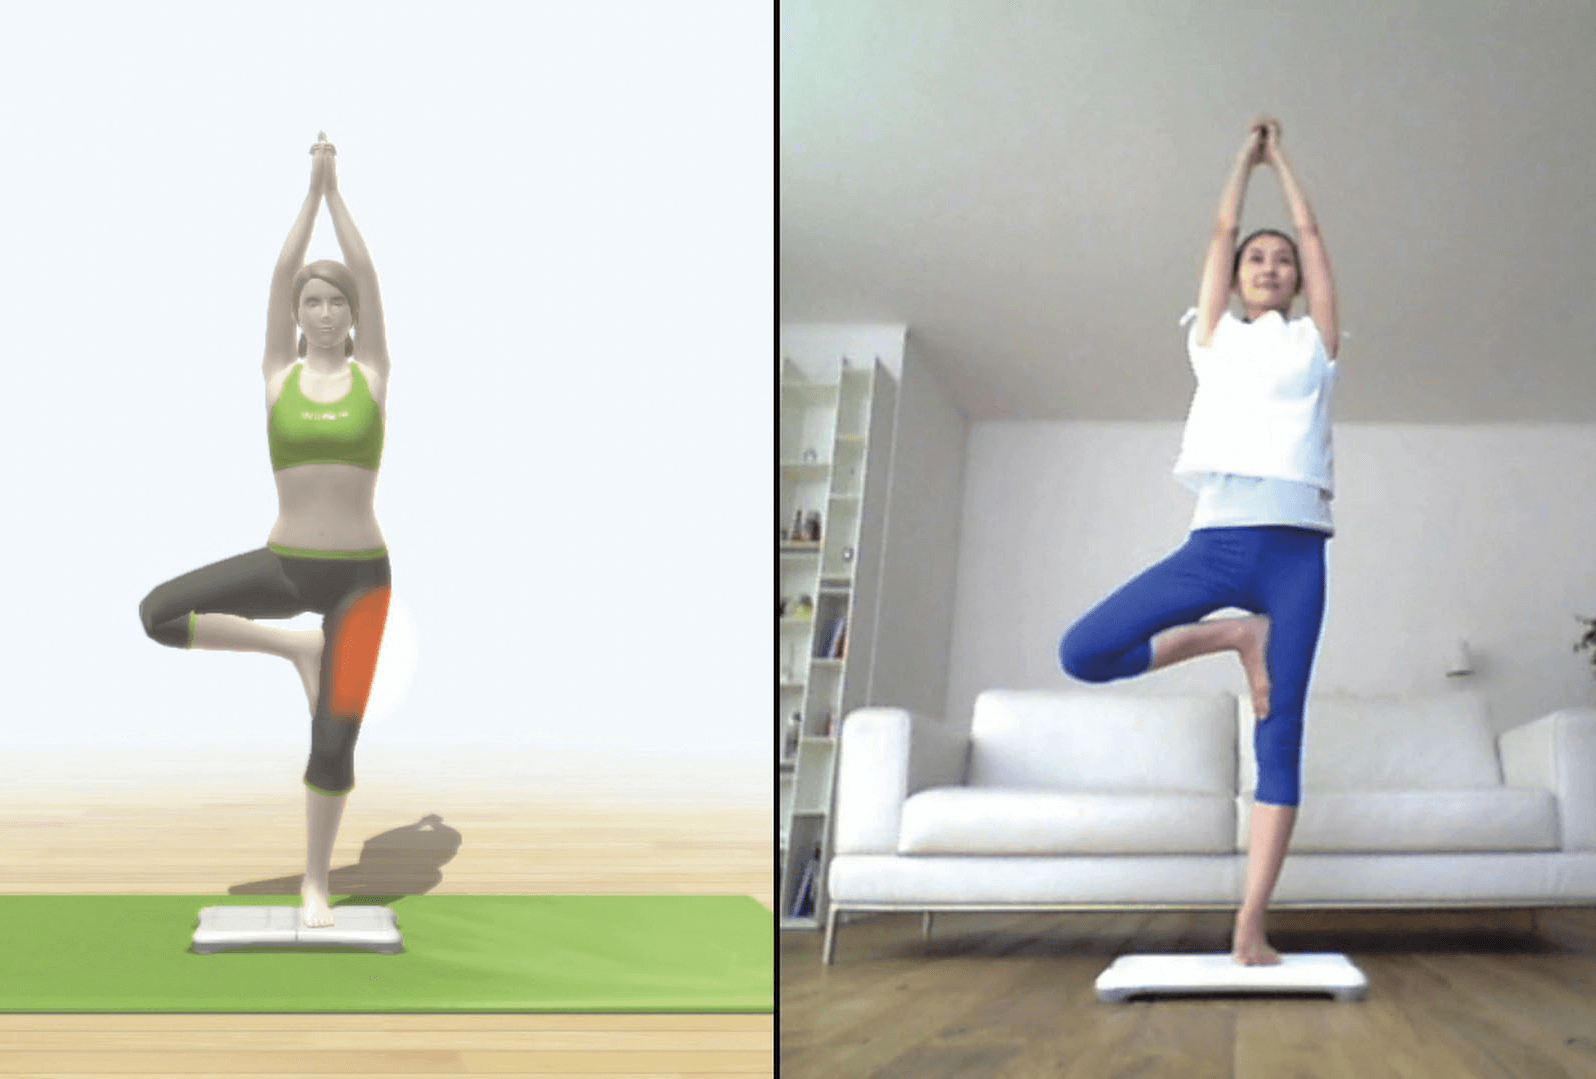
\includegraphics[width=0.75\textwidth]{Images/ExistingGames/WiiFit_Pose.png}
    \caption{A person doing yoga exercise alongside an in-game avatar.}
    \label{fig:wii_fit_pose}
\end{figure}

The additional controller is called the Wii Balance Board \citep{ign_wii_2008} and is one reason this game can be categorized as alternative. The board’s purpose is to track the player's movement and translate it to the player’s in-game avatar, as seen in Figure \ref{fig:wii_fit_pose}. A bathroom weight inspired the board’s design, and it consists of four weight sensors, one in each corner. The controller connects to the console through Bluetooth, where it calculates the player's movement in real-time \citep{jacquot_how_2010}. Based on the player’s motion, the game gives feedback on how the exercise is going, as seen in Figure \ref{fig:wii_fit_pushup}.

\begin{figure}[H]
    \centering
    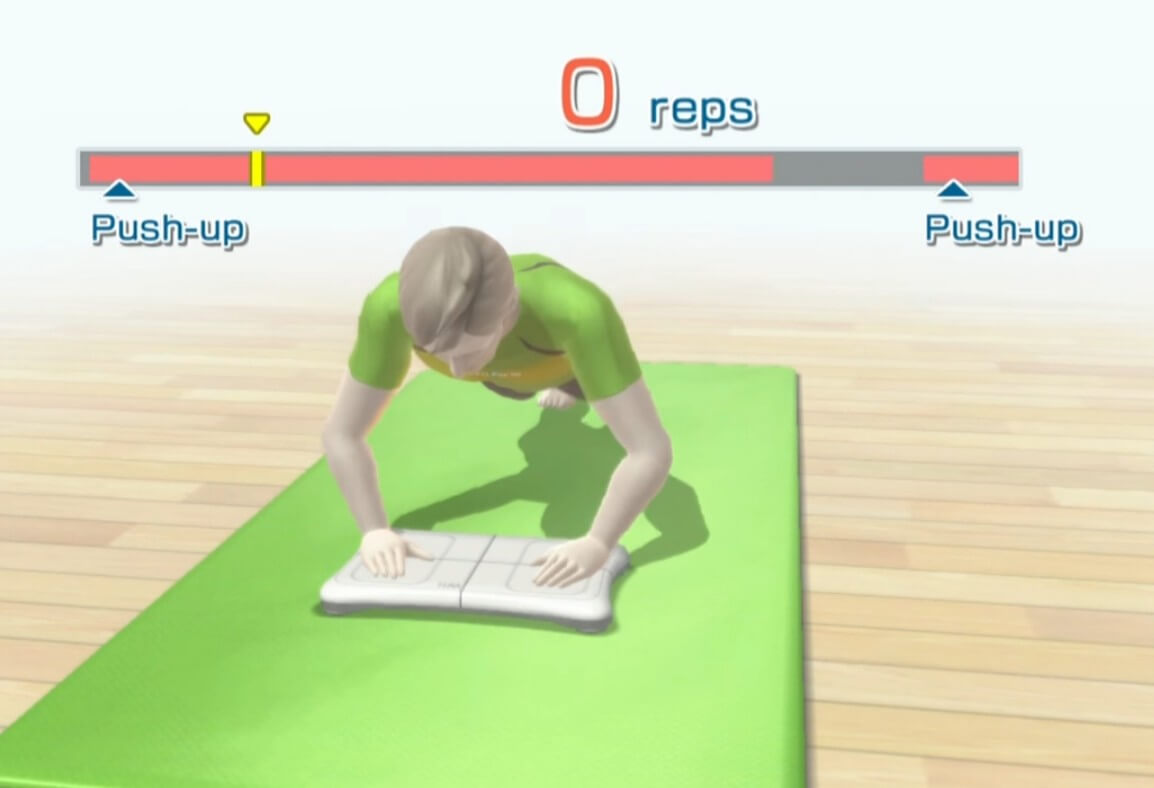
\includegraphics[width=0.75\textwidth]{Images/ExistingGames/WiiFit_Pushup.jpg}
    \caption{Screenshot of the in-game avatar using the board to track push-ups.}
    \label{fig:wii_fit_pushup}
\end{figure}

In addition to the alternative input, Wii Fit is also a gamification concept exercising. The game’s goal is to create a fun way to get in shape from the comfort of the player’s home. Nintendo brings a comprehensive set of games that are engaging for the entire family with individual progress so all players can compare themselves against each other.

Wii Fit was initially designed as an interactive health and fitness experience for the general public. However, Wii Fit’s benefits have been studied in many clinical settings, such as in multiple sclerosis patients and stroke patients\citep{tripette_contribution_2017}. A 2011 study of the health and wellness benefits of Wii Fit on university students revealed a significant change in body mass index, weight, and intrinsic and total motivation for its participants\citep{jacobs_wii_2011}.

\subsection{Mosquito Mania}
Mosquito Mania is a game concept developed at NTNU in connection with a music technology bachelor thesis in 2012. The game was developed as an attempt to create a new way of entertaining people by using audio stimulation and concepts from game development.

The primary purpose of the game is to kill as many mosquitos as possible within 60 seconds. An 8-32 array of speakers is positioned in a circle around the player, emitting mosquito sounds in a 2-dimensional space, as seen in Figure \ref{fig:mosquito_mania_anonym}. The player is then assigned the task of killing the mosquitos using a custom-made gun-like controller, measuring the direction it is pointed. A microcontroller combined with an accelerometer, compass, and gyroscope is mounted on the controller. Though the game primarily focuses on audio, the game has a dashboard for game statistics and scoreboard (see Figure \ref{fig:mosquito_mania_dashboard}).

\begin{figure}[H]
    \begin{minipage}[t]{.475\textwidth}
        \centering
        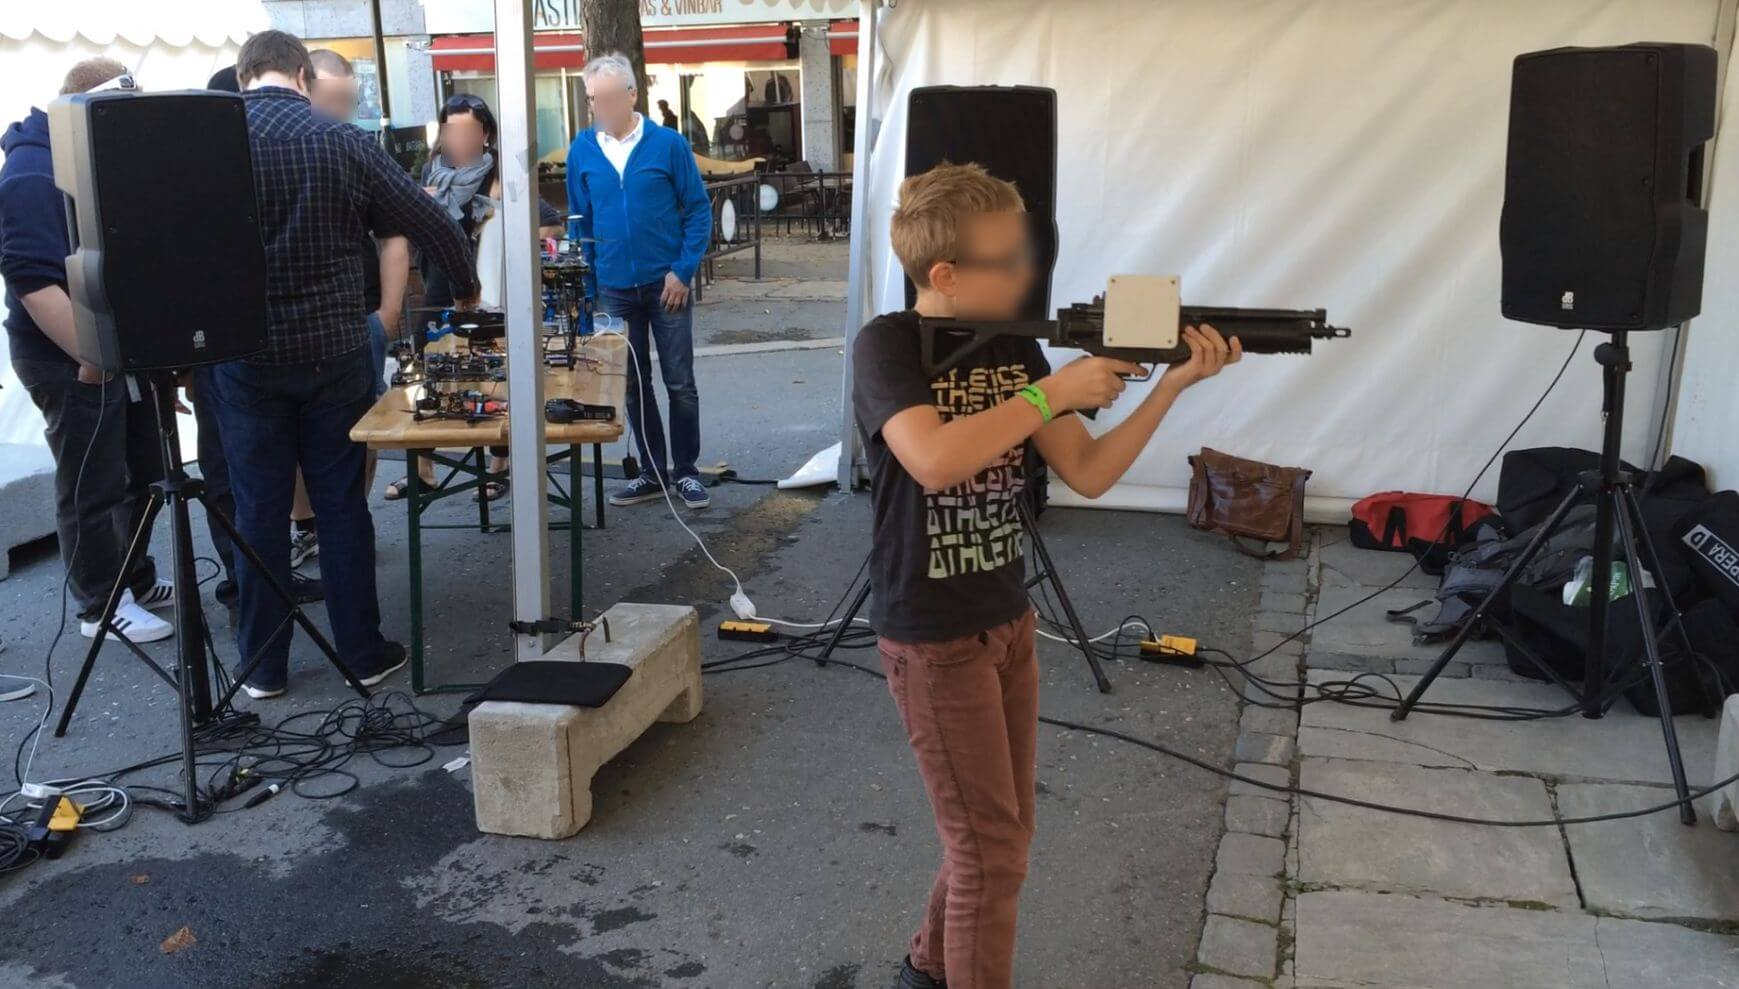
\includegraphics[width=\textwidth]{Images/ExistingGames/MosquitoMania_anonym.jpg}
        \caption{A person playing Mosquito Mania.}
        \label{fig:mosquito_mania_anonym}
    \end{minipage}
    \hspace{0.05\textwidth}
    \begin{minipage}[t]{.475\textwidth}
        \centering
        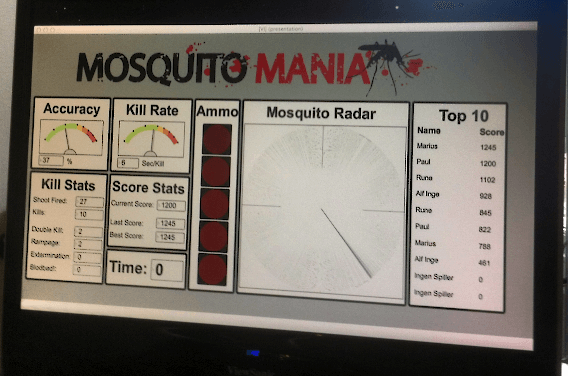
\includegraphics[width=0.87\textwidth]{Images/ExistingGames/MosquitoMania_Dashboard.png}
        \caption{Mosquito Mania’s game dashboard with game statistics and leaderboard.}
        \label{fig:mosquito_mania_dashboard}
    \end{minipage}
    \vspace*{-\baselineskip}
\end{figure}

The game is an alternative for multiple reasons. First of all, it uses an alternative input source, i.e., the custom controller for playing. This unique controller could by itself contributed to categorize the game as alternative. However, the primary reason for Mosquito Mania to be an alternative game is the unusual approach of using audio as the primary output source. Regular games typically combine sounds and music as a secondary output source in addition to visual feedback. The game concept is unique, and by removing the visual aspect, a new twist is introduced to the game. Even though the game was not developed for any special target groups, it became immensely popular among people with visual impairment \citep{gran-jansen_mosquito_2020}.

\clearpage

\section{Comparison of Existing Alternative Games}
\label{chap:comparison_of_existing_games}

To compare the alternative aspects of all the games mentioned in the previous chapter, the alternative games model presented in Chapter \ref{chap:what_is_alternative_game} has been used. It provides a quick overview of how the game differs and presents concrete characteristics for all the games in each of the six categories. The model in Table \ref{tab:existing_games} is a simplified version of the complete model found in Appendix \ref{appendix:complete_model} where the unused rows have been omitted for readability.

\begin{table}[H]
    \centering
    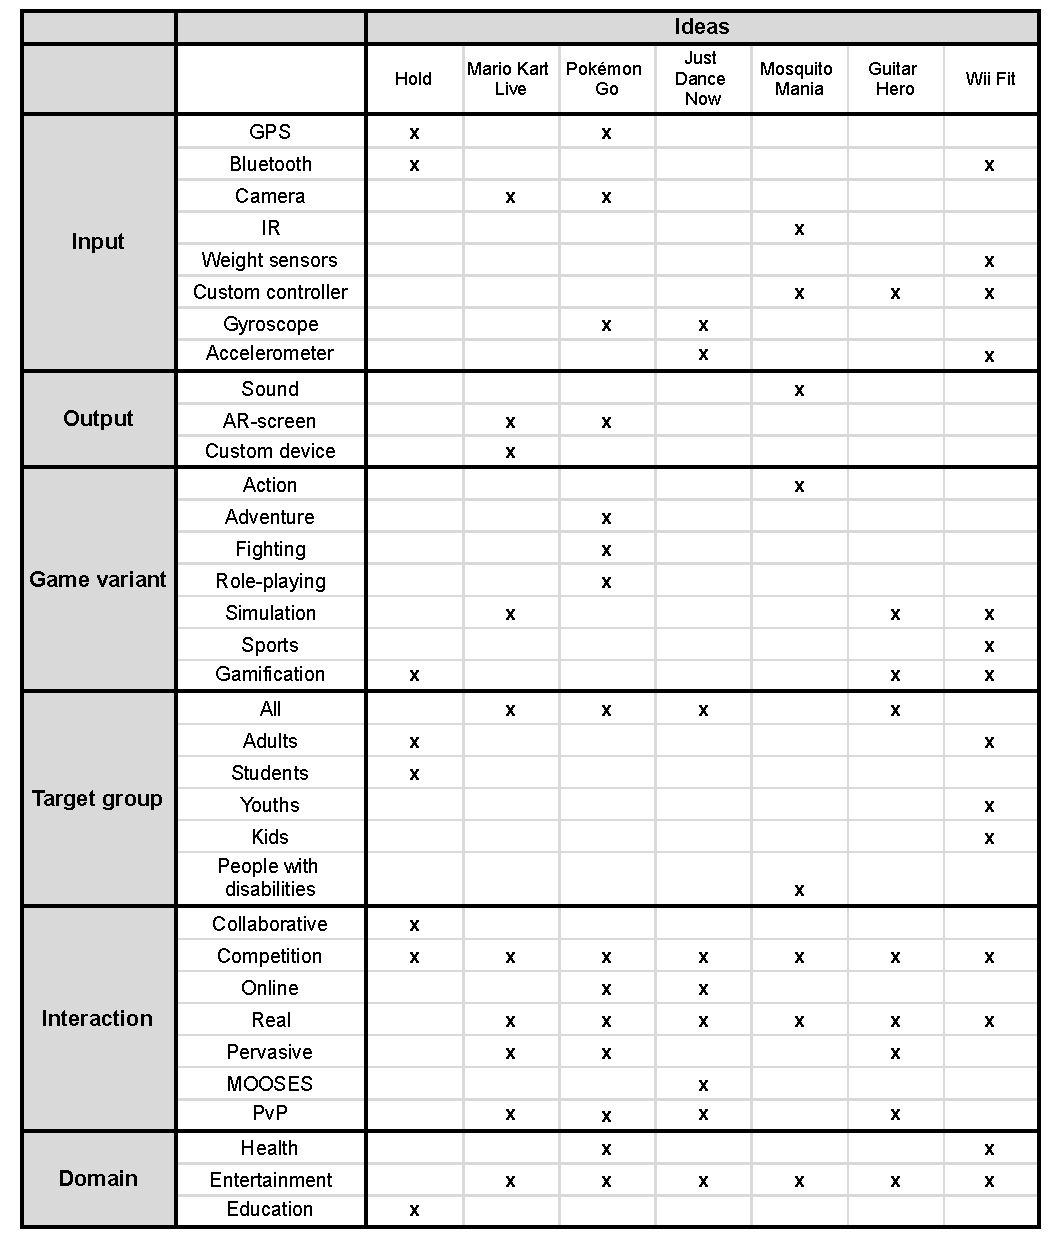
\includegraphics[width=0.9\textwidth]{Images/Models/ExistingGames.pdf}
    \caption{Existing alternative games characteristics}
    \label{tab:existing_games}
\end{table}

\subsection{Analysis of Input}
The first section of the model shows a wide range of \textit{input} types used in the games.  The variation is likely to come from the fact that many games are developed for a mobile platform. Mobile phones today include various input sensors that can be used to create alternative game concepts. GPS, Bluetooth, gyroscope are examples of such sensors. 

The games Hold, Pokémon Go, and Just Dance Now are totally or partially developed for mobile platforms. Hold and Pokémon Go uses the device’s GPS to use the context of the player’s location in the game. The location-aware feature creates a better in-game experience, and players are forced to move to unlock certain features. Pokémon Go and Just Dance Now both take advantage of the phone’s gyroscope. The gyroscope can detect rotation, telling a game how the mobile device is positioned in the real world. Just Dance Now also uses the accelerometer to track the player’s movement while dancing. The use of both gyroscope and accelerometer determines if the player is doing the right move at the right time, providing a fun and immersive player experience.

In the early days of computer games, custom controllers for each game were common \citep{overmars_brief_2012}. Using different controllers was adverse for the players because it forced them to buy new ones for every game. Furthermore, non-custom controllers can cause a poor user experience if it does not have an optimal or logical design. Nowadays, custom controllers are rare, and games are often produced for specific consoles rather than unique controllers. However, there exist games today with custom controllers, and Guitar Hero, Wii Fit, and Mosquito Mania are all examples of this. In these games, it makes sense to use a custom controller more suited for the game's purpose since a regular game controller would make it hard to create a realistic game. Using a special controller as input is a classic example of an alternative game.

\subsection{Analysis of Output}
The second section of the model looks at the alternative use of \textit{output} in games. Even though today’s games often use sound effects and music, this does not make them alternative. The use of sound in Mosquito Mania is more alternative as it is the only output. The game focuses on the player's ability to sense the sound's direction, which is an alternative way of challenging the player's hearing instead of the eyesight.

Furthermore, Pokémon Go and Mario Kart Live use the camera as an input to produce an Augmented Reality (AR) output. AR technology is alternative in games because projecting artificial objects onto the real world is based on interpreted input. In both games, players use a handheld device. AR in mobile devices is more available to the consumers but creates a less immersive gaming experience than an AR headset.


\subsection{Analysis of Game Genre}
A selection of \textit{game genres} is listed in the third section of the table. These game genres themself do not make games alternative. However, they do tell something about what type of game it is. There is one exception to this: gamification. Gamification is alternative because it gamifies activities and tasks to make them fun and engaging while motivating the player. Hold, Guitar Hero, and Wii Fit are all gamification concepts. Hold gamifies and rewards players for putting the phone down, Guitar Hero gamifies playing the guitar, and Wii Fit gamifies and motivates working out. Furthermore, games can also be classified within multiple genres, making the game more alternative. However, this is not implied.

\subsection{Analysis of Target Group}
The identified \textit{target groups} can be found in the fourth section of the model. All games have one or more dedicated target groups, corresponding to everyone or a distinguished set of users. The target groups might overlap or intersect; for instance, students and young adults intersect. Mario Kart Live, Just Dance Now, and Guitar Hero are examples of games where the target group is “all”. Still, these games might be more addressed towards a younger crowd. Mosquito Mania is also a game that most people can play; however, it is especially applicable for people with visual impairment who may have trouble playing ordinary games.

\subsection{Analysis of Interaction}
The fifth section of the model displays the types of \textit{interactions} that have been identified in the existing games studied in Chapter \ref{chap:existing_games}. Interaction types can be found in all ordinary games and do not imply that a game is alternative. However, how the interaction is accomplished may be categorized as alternative.. All seven games use a combination of interaction methods, and all games include some degree of interaction through competition. Competition can be conducted in numerous ways, e.g., by utilizing a scoreboard. Just Dance Now offers, like many other games, different player modes. Players can play alone, against friends in the same physical or virtual room in real-time, or online through the global scoreboard. These gameplay variations make the game very flexible, and players can play in the way they want. The other games offer similar but not so extensive features as Just Dance Now. Mario Kart Live, Pokémon Go, and Guitar Hero all include the competitive elements of PvP interaction. In these games, players communicate in the real world, but the gameplay happens in the virtual world.

Hold is the only game that includes a collaborative mode where players can connect their device with their friends’ to boost points. If one player quits, the player will not only lose his or her focus but also stop the boosting for the collaborating players. This interaction feature is likely to strengthen the player’s motivation for not using their phones. 


\subsection{Analysis of Domain}
The sixth and last section of the model displays the \textit{domain} of the games. Traditionally speaking, games often belong to the domain of entertainment, and therefore the use of other domains can classify a game as alternative. The exercise game Wii Fit is directly connected to the domain of physical health. Pokémon Go also exploits the benefits of physical health from having players move around. Hold is not like a traditional game and thus classifies only in the educational domain since its primary target group is students.

\subsection{Summary}
This chapter has focused on showcasing multiple different and typical examples of alternative games (based on our definition presented in Chapter \ref{chap:what_is_alternative_game}). The examples have been shortly described and compared with each other to highlight their differences. A table with the characteristics of each game has been presented and analyzed. The next chapter will shift the focus from the concept to the technical aspect of alternative games.  

\clearpage

\section{Technology Review}
\label{chap:technology_review}
In this chapter, we will study technology relevant to the development of alternative games, increasing our understanding of the possibilities in this field. The learning will come in handy when we are going to invent new alternative game concepts and later when we are going to develop our chosen concept.

The diversity of alternative games today is considerable. Based on our definition from Chapter \ref{chap:what_is_alternative_game}, many games can be categorized as alternative. A few examples were given in Chapter \ref{chap:existing_games}, but many more exist. Because there are numerous unique alternative game concepts, there are also a lot of variations in the technology they use. Thus covering everything is outside the scope of this project. Therefore, we decide to focus on the type of technology that is directly relevant to us. As described in our motivation in Chapter \ref{chap:motivation}, our goal is to create an application that can reach as many users as possible. As a consequence of this, we will mainly consider mobile development tools. However, we will first briefly examine the possibilities of technology that alternative games explore today.

\subsection{Diversity in Alternative Game Technology}

\begin{wrapfigure}{r}{0.5\textwidth}
    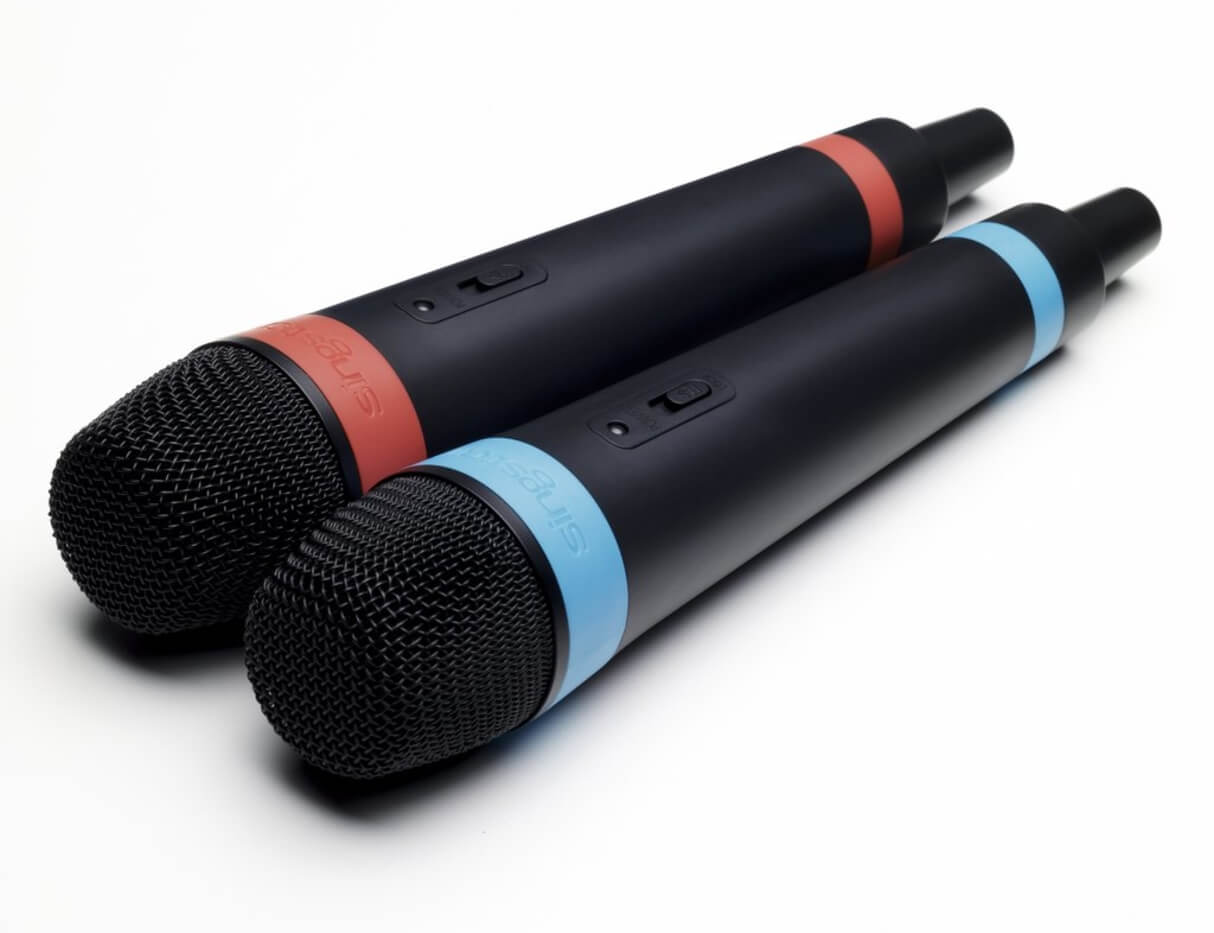
\includegraphics[width=0.4\textwidth]{Images/TechnologyReview/SingstarController.jpg}
    \centering
    \caption{Singstar microphones.}
    \label{fig:singstar}
    \vspace*{-1\baselineskip}
\end{wrapfigure}

The technology used in alternative games can, in principle, consist of almost anything. The limits in what can be done are often affiliated with the game developers’ imagination rather than the technology. A common way of creating alternative games, as described in the model in Chapter \ref{chap:what_is_alternative_game} is to explore custom-designed input or output devices. A typical example is a specific controller custom-designed for the game. Alternative games often bundle the game together with the needed controller. A concrete example of such a game is Singstar, a karaoke game where players compete to get the highest score by hitting as many notes as possible. The game includes a custom microphone, as seen in Figure \ref{fig:singstar}, that the players use when singing. By using this microphone, the player gets an increased real-world experience. Some other examples of games that use custom controllers as input are Wii Fit, Guitar Hero, and Mosquito Mania, all of which were described in Chapter \ref{chap:existing_games}. 

Augmented Reality (AR) and Virtual Reality (VR) are examples of technologies where uncommon input and output are used. The technologies have become increasingly popular in the last couple of years and are expected to continue to be available to more people in the coming years as well \citep{petrock_us_2020}. Both technologies are great platforms for developing alternative games.

VR is a technology based on simulating an environment for users where they become a part of that virtual experience. The situation could be based on a simulated version of the real world or an imaginary one. VR games give another level of immersion in the game because everything the player sees is dependent on the fictional environment. Consequently, more parts of the game experience can be controlled by the developer. An example of a player immersed in a VR game can be seen in Figure \ref{fig:playing_vr}. The corresponding in-game look for the player could be similar to the view in Figure \ref{fig:gameplay_vr}. The screenshot is captured from an actual game-play session in “The Climb” for Oculus Quest, a popular VR headset. 

\begin{figure}[H]
    \begin{minipage}[t]{.52\textwidth}
         
\includegraphics[width=0.84\textwidth]{Images/TechnologyReview/OculusQuest.jpg}
        \centering
        \caption{A person playing VR games using Oculus Quest 2.}
        \label{fig:playing_vr}
    \end{minipage}
    \hspace{0.05\textwidth}
    \begin{minipage}[t]{.43\textwidth}
        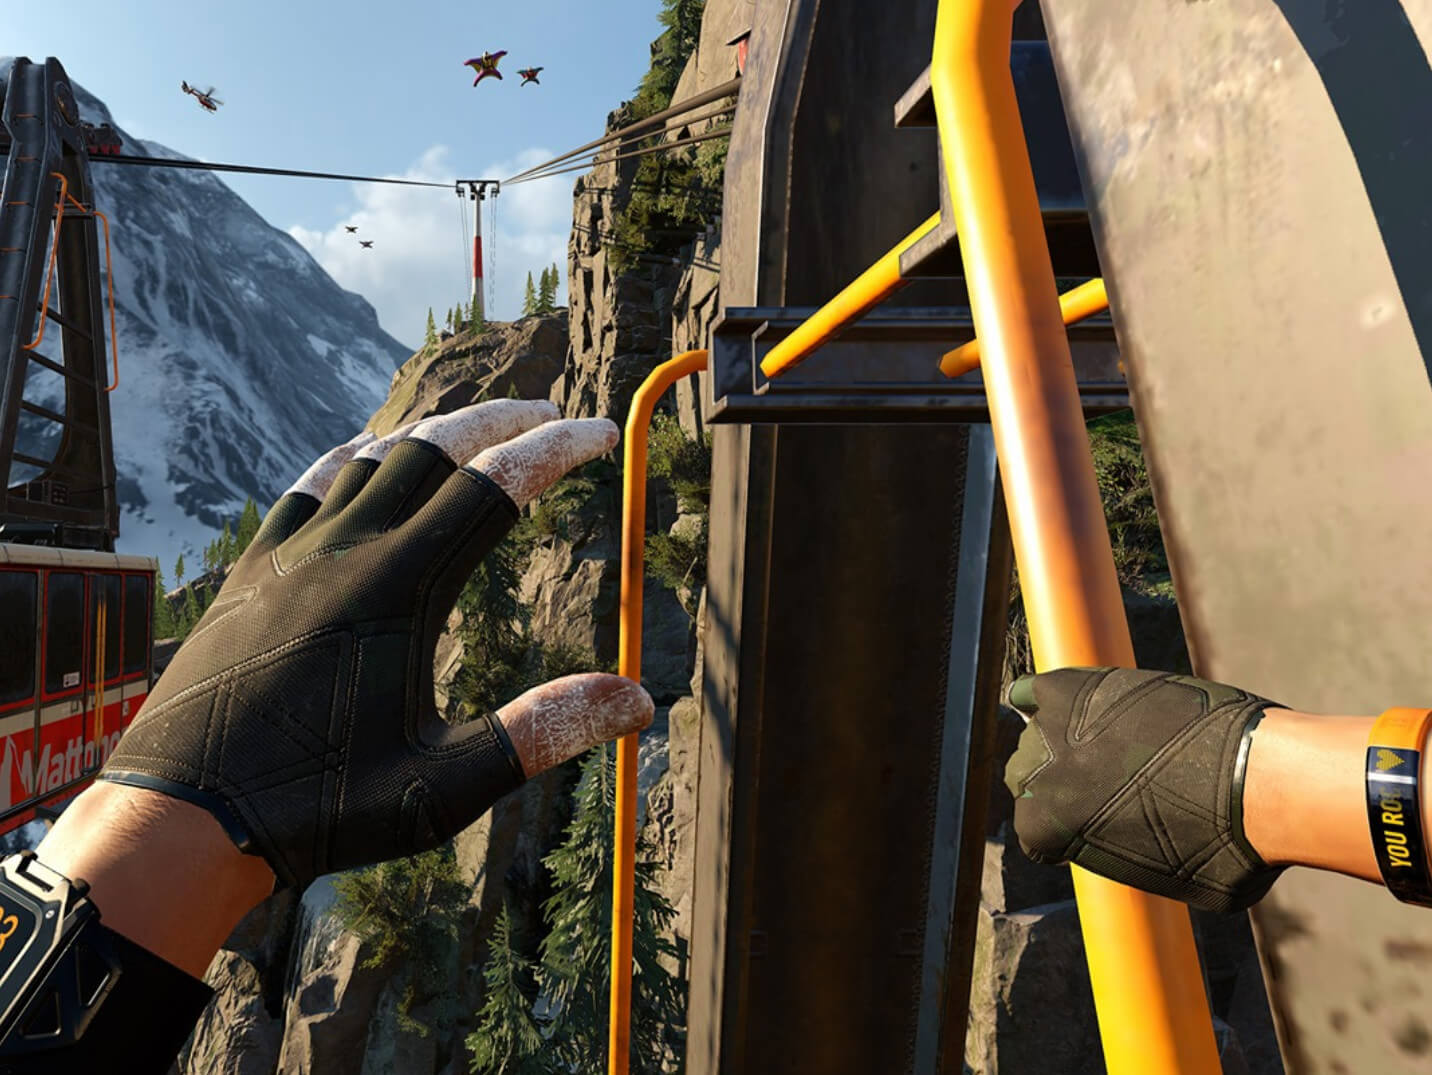
\includegraphics[width=0.8\textwidth]{Images/TechnologyReview/TheClimbOculus.jpg}
        \centering
        \caption{Screenshot of Oculus Quest gameplay from The Climb.}
        \label{fig:gameplay_vr}
    \end{minipage}
\end{figure}

AR is similar to VR, but instead of projecting elements to a simulated environment, AR uses the real world. Simulations can be created using specially developed glasses, as illustrated in Figure \ref{fig:ar_glasses}, or more commonly, with a mobile phone screen and camera. Similar to VR, AR creates another game experience than regular games. One of the most common examples of an AR game is Pokémon Go, described in Chapter \ref{chap:existing_games}.

\begin{figure}[H]
    
\includegraphics[width=0.8\textwidth]{Images/TechnologyReview/ARGlasses.jpeg}
    \centering
    \caption{AR projections in the real world using glasses.}
    \label{fig:ar_glasses}
\end{figure}

In addition to using custom controllers, AR, and VR, mobile phones are commonly used to develop alternative games. Mobile devices have a lot of sensors that developers can utilize to create a game. Also, mobile applications’ distribution is relatively simple because the popular operating systems have pre-made tools for distributing applications. The simplicity of distribution makes it more likely for users to download an application to their mobile phone than they are to buy some kind of custom device only for that game.

As mentioned in the motivation, we have focused on developing a concept that can reach as many users as possible. Mobile technology is by far the easiest and most available way to do this today. Therefore, the rest of this technology review will focus on which tools can be utilized to create the best mobile applications. The content presented in the rest of the chapter is used later to decide how we will develop our application.

\subsection{Mobile Application Development Tools}
Today, most smartphones on the market use Android or iOS as their operating system \citep{statcounter_mobile_2020}. The development can be done mainly in two different ways: native or using a cross-platform framework. The native development method uses the APIs and languages provided by Apple or Google. The cross-platform framework method uses third-party tools for creating an application that can be run on both platforms. There are strengths and weaknesses in using either of the approaches, which should be carefully considered before choosing one of them. Early decisions affect evolvability and can be hard or costly to change later \citep{ford_building_2017}. 

Alternative games often utilize the mobile phone’s sensors, such as GPS, Bluetooth, and gyroscope, as a central aspect of the game. It is, therefore, essential that the frameworks considered for alternative games have good support for accessing data from these sensors. Obtaining data from the devices is not an issue in the native approach since they are continuously updated with the latest and most detailed data available to the developer.

\subsubsection{Native Solutions}
The obvious drawback of using the native approach is that Android and iOS applications need to be developed separately. Since the native solutions for Android and iOS are based on two different programming languages, Java and Swift, code cannot be shared between both applications. The developers then have to implement and maintain both solutions, resulting in a “doubled” work amount.

The main strength of the native solution is that you always have access to the latest and greatest APIs provided by the companies developing the operating systems. Every time a new OS gets released, the developers have access to the latest features instantly. Availability of new features can be valuable for developers when working with special features that are not commonly utilized and creates a faster implementation loop when new features become available.

Another strength of the native solution is maturity. The APIs and tools provided are usually well documented and tested. Developing an application using this approach is not dependent on third-party developers writing documentation and updating their framework. 

If performance is critical for the application, the native approach is also preferred. While different frameworks’ performance varies significantly, based on what operations are done, native solutions are usually more performant than cross-platform frameworks \citep{biorn-hansen_empirical_2020}.

\subsubsection{Cross-Platform Solutions}
There are several variants of cross-platform solutions for mobile applications, each with different strengths and weaknesses. In this section, we will consider general-purpose and game-focused frameworks. The primary benefit of all of these approaches is the ability to share codebase between the Android and iOS applications. In theory, this should decrease development and maintenance costs since the developers can focus on only one framework. Another benefit of using cross-platform solutions is that they often utilize other languages than those supported by Google and Apple. Consequently, a developer can choose a language that fits better to their expertise.

General cross-platform frameworks focus on creating a simple application that can run on both Android and iOS. The different frameworks have their own approach, but they provide similar services. Three of the most known frameworks are React Native, Flutter, and Xamarin. When deciding on which general-purpose framework one should choose, the developer preferences are often central. But of course, it is necessary to make sure the framework supports what you plan to do in the application. General cross-platform application frameworks are suitable for most applications that do not include too much complicated graphics.

Game focus mobile framework focuses more directly on creating applications with 3D elements. The frameworks provide tools that make the creation of game elements and complex visualization easier. Thus they are perfect when working with this. However, they might be unnecessarily complex and not fit for developing applications that are simpler graphically. Two of the best-known examples of game-focused mobile frameworks are Unity and Unreal Engine.

\subsubsection{Choosing Between Native and Cross-Platform}
So whether a native approach or a cross-platform approach is best essentially comes down to the situation. If performance and access to the latest and greatest the operating system can offer, a native solution is preferable. If a shared codebase between Android and iOS or minimizing development time is crucial, a cross-platform solution is probably the way to go. And last, if you are developing 3D intensive applications, a game-specific framework should be the preferred option.

\subsection{Data Solutions}
An important aspect of game development is how the data should be stored and managed. The social element in games is crucial to create an enjoyable experience for the player \citep{sweetser_gameflow_2005}. A way of authenticating users and a central storing mechanism to keep player data is essential to provide this. There are many approaches to do this. 

Previous to cloud services, writing a custom API that handled requests from the application was the way to go. However, in the last couple of years, cloud service solutions called Backend as a Service (BaaS) are frequently used in mobile applications. The idea here is that the solution should provide all necessary backend solutions for mobile applications. All the big cloud providers, Microsoft, Google, and Amazon, offer this kind of service.

\subsubsection{Backend as a Service (BaaS)}
As mentioned above, BaaS provides all the necessary backend services for a mobile application, including authentication, storage, insights, and more. Such a solution is supposed to simplify mobile application development since the developers do not need to spend much energy on planning, creating, and maintaining a custom backend. They can instead focus on improving the application. All the big cloud providers, Microsoft, Google, and Amazon, offer similar services with Azure Mobile Apps, Firebase, and AWS Amplify, respectively. Choosing between these is usually subjected to taste and preferences, but the mobile application’s technology could influence the choice. For example, if Xamarin is used as a mobile application tool, Azure Mobile Apps is a great fit because Microsoft provides both. Consequently, the developer gets a lot “for free.”

In addition to the solutions from the big cloud service providers, there exist other alternatives that could be used as a replacement or extension. Two of the ones that caught our interest during this work are Parse and Hasura. Parse is an open-source backend framework. It aims to create a more straightforward backend development process and has a large community base. Parse could be a great alternative to Azure Mobile Apps, Firebase, or AWS Amplify. Hasura is a more specialized database solution. The service provides a PostgreSQL database with a GraphQL API and built-in authentication. The main selling point for Hasura is the use of GraphQL, as opposed to the more common REST style. The main benefit of using GraphQL is the ability to specify which data properties you want to fetch, limiting the amount of data transferred, and thus is perfect for mobile applications. Hasura is not a complete BaaS and probably needs to be used in coherence with another service.

\subsubsection{Custom API}
The next approach for creating a backend solution is to write a custom API. Developing such a system is a widespread solution and was the preferred one for almost all client-server-based applications for a long time. By creating a custom API, the developer can tailor the system for the application’s needs. It is also simpler to integrate a custom API with an existing system if that is a requirement. 

There exist a large diversity of different frameworks for creating a custom API. In general, all major languages have at least one tool for developing a web API. Examples of some tools are Flask in Python, ASP.NET in C\#, and Express in Node.js.

\subsubsection{Choosing Between BaaS and Custom API}
The choice of backend solutions often depends on the developers’ preferences. If the application’s goal is to create something that does not require a lot of business logic and a complex backend, BaaS is probably the way to go. A custom API may be the best solution for larger companies where the backend needs to integrate with the existing system and contain complex logic.

\subsection{Summary}
This chapter started by briefly looking at today’s diversity in the technology used in alternative games. After that, relevant mobile application development tools were discussed and compared. This knowledge will be helpful when deciding on how the application should be developed. As explained in the motivation in Chapter \ref{chap:motivation}, we want to create a game that should “be available to as many users as possible.” Thus, a cross-platform mobile application with a BaaS data solution will probably be the preferred solution. Chapter \ref{chap:chosen_technologies} presents more concrete details on which tools we chose and why they were selected.
\clearpage

\section{Ideas for New Alternative Games}
\label{chap:new_ideas}

In this chapter, a description and evaluation of six alternative game concepts invented during our prestudy work will be presented. Previously (in Chapter \ref{chap:what_is_alternative_game}), we have defined and constructed a model to establish what an alternative game is. The model was used to develop new ideas, as illustrated in Figure \ref{fig:new_ideas_process}. Starting with a loose idea and then tweaking the characteristics made us invent new concepts that we otherwise would not have considered. This process is a generalized approach that can generate alternative games from ideas that are initially regular games or as an iterative process to add more alternative features.

\begin{figure}[H]
    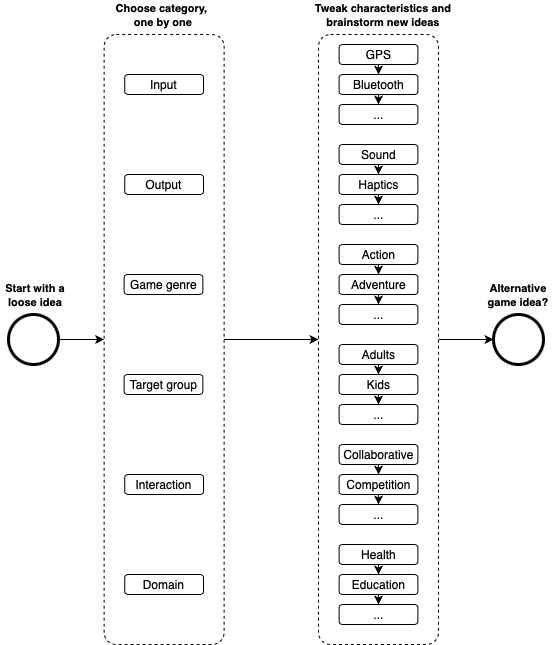
\includegraphics[width=0.8\textwidth]{Images/NewIdeas/NewIdeasProcess.png}
    \centering
    \caption{Inventing new ideas with our alternative games model}
    \label{fig:new_ideas_process}
\end{figure}

Later, we studied literature explaining how to create an enjoyable game, reward systems, and player types in chapters \ref{chap:design_an_enjoyable_game}, \ref{chap:reward_systems}, and \ref{chap:player_types}. The knowledge obtained from this work gave us insight into game design. Finally, Chapter \ref{chap:existing_games} gave us an overview of existing alternative games. This research showed us examples of the current possibilities and stimulated our fantasy to invent even more ideas.

After outlining and evaluating the six ideas, the model defined in our prestudy will be used to compare them. This comparison will, similar to Chapter \ref{chap:existing_games}, help us describe the differences between the games and why they characterize as alternative.

Our primary motivation for choosing this specific task was the opportunity to create an application with a socially beneficial purpose. The concepts should preferably introduce something valuable to society while still exploring the genre of alternative games. Also, the goal was to make the application available to as many users as possible. Based on these factors, we decided early that the game had to be based on the mobile platform. Consequently, the concepts described later in this chapter are invented with this in mind. Over three billion people own a smartphone today \citep{odea_smartphone_2020}. By targeting the smartphone market and these two operating systems, we can reach many potential users. Furthermore, smartphones have a variety of sensors that can be used in alternative games.

Another important consideration during the invention process was that the concept needed to be easy to test. The application’s testability is an essential consideration when we are going to develop our chosen concept. We want to find out how people are using the application and whether or not they are enjoying it.


\subsection{Hover}
\label{sec:hover}
The first alternative game idea we invented is named Hover. The concept is inspired by the existing application \textit{Hold}, described in Chapter \ref{chap:existing_games}. In short, players get points in Hold for not using their phones. Hover uses the same principle, but the points are awarded based on their location. Meaning the players get points when they are located at certain spots in the real world. The points can result in awards and achievements. As discussed in Chapter \ref{chap:reward_systems}, rewards create positive experiences for players and improve the game’s enjoyability.

The spots are based on areas that could improve a person’s well-being, such as training centers, schools, libraries, museums, and art galleries. The locations are classified corresponding to their purpose, e.g., \textit{exercise}, \textit{education}, and \textit{culture}. For example, training centers will be categorized as health, schools as knowledge, and museums as culture. The rewards and points will be summarized both for the individual categories and to a total score. In this way, the players can focus on doing their best in a specific category or getting the best overall score.

A crucial part of the game concept is to get people to use the application. The social interaction in the game is an important aspect to achieve that. One way of doing this is by introducing more points if a player is using the application while being together with friends. For example, if two or more players study together, they get double the amount of points. This aspect is particularly relevant in today’s situation with the COVID-19 pandemic in the world. Papers are suggesting that more people are struggling with loneliness \citep{groarke_loneliness_2020}. The application can contribute to improving mental health by motivating people to engage socially.

The game’s social aspect is also essential to increase player enjoyment in the game, as described in the GameFlow article in Chapter \ref{chap:design_an_enjoyable_game}. One way of encouraging competition is to introduce challenges where the players can compete against each other. An example of a challenge could be “first person to get 1000 points”. Another way of encouraging competition is a high score list, enabling players to compare themselves against others.

The game concept can be more enjoyable for the players by including elements of fantasy, as discussed by Malone (see Chapter \ref{chap:design_an_enjoyable_game}). A suggestion here is to include a virtual character that evolves depending on the number of points the player has earned during a period, e.g., the last 30 days, for the different categories. An example of how the virtual character could evolve when improving the health category is illustrated in Figure \ref{fig:player_evolement} below. 

\begin{figure}[H]
    \centering
    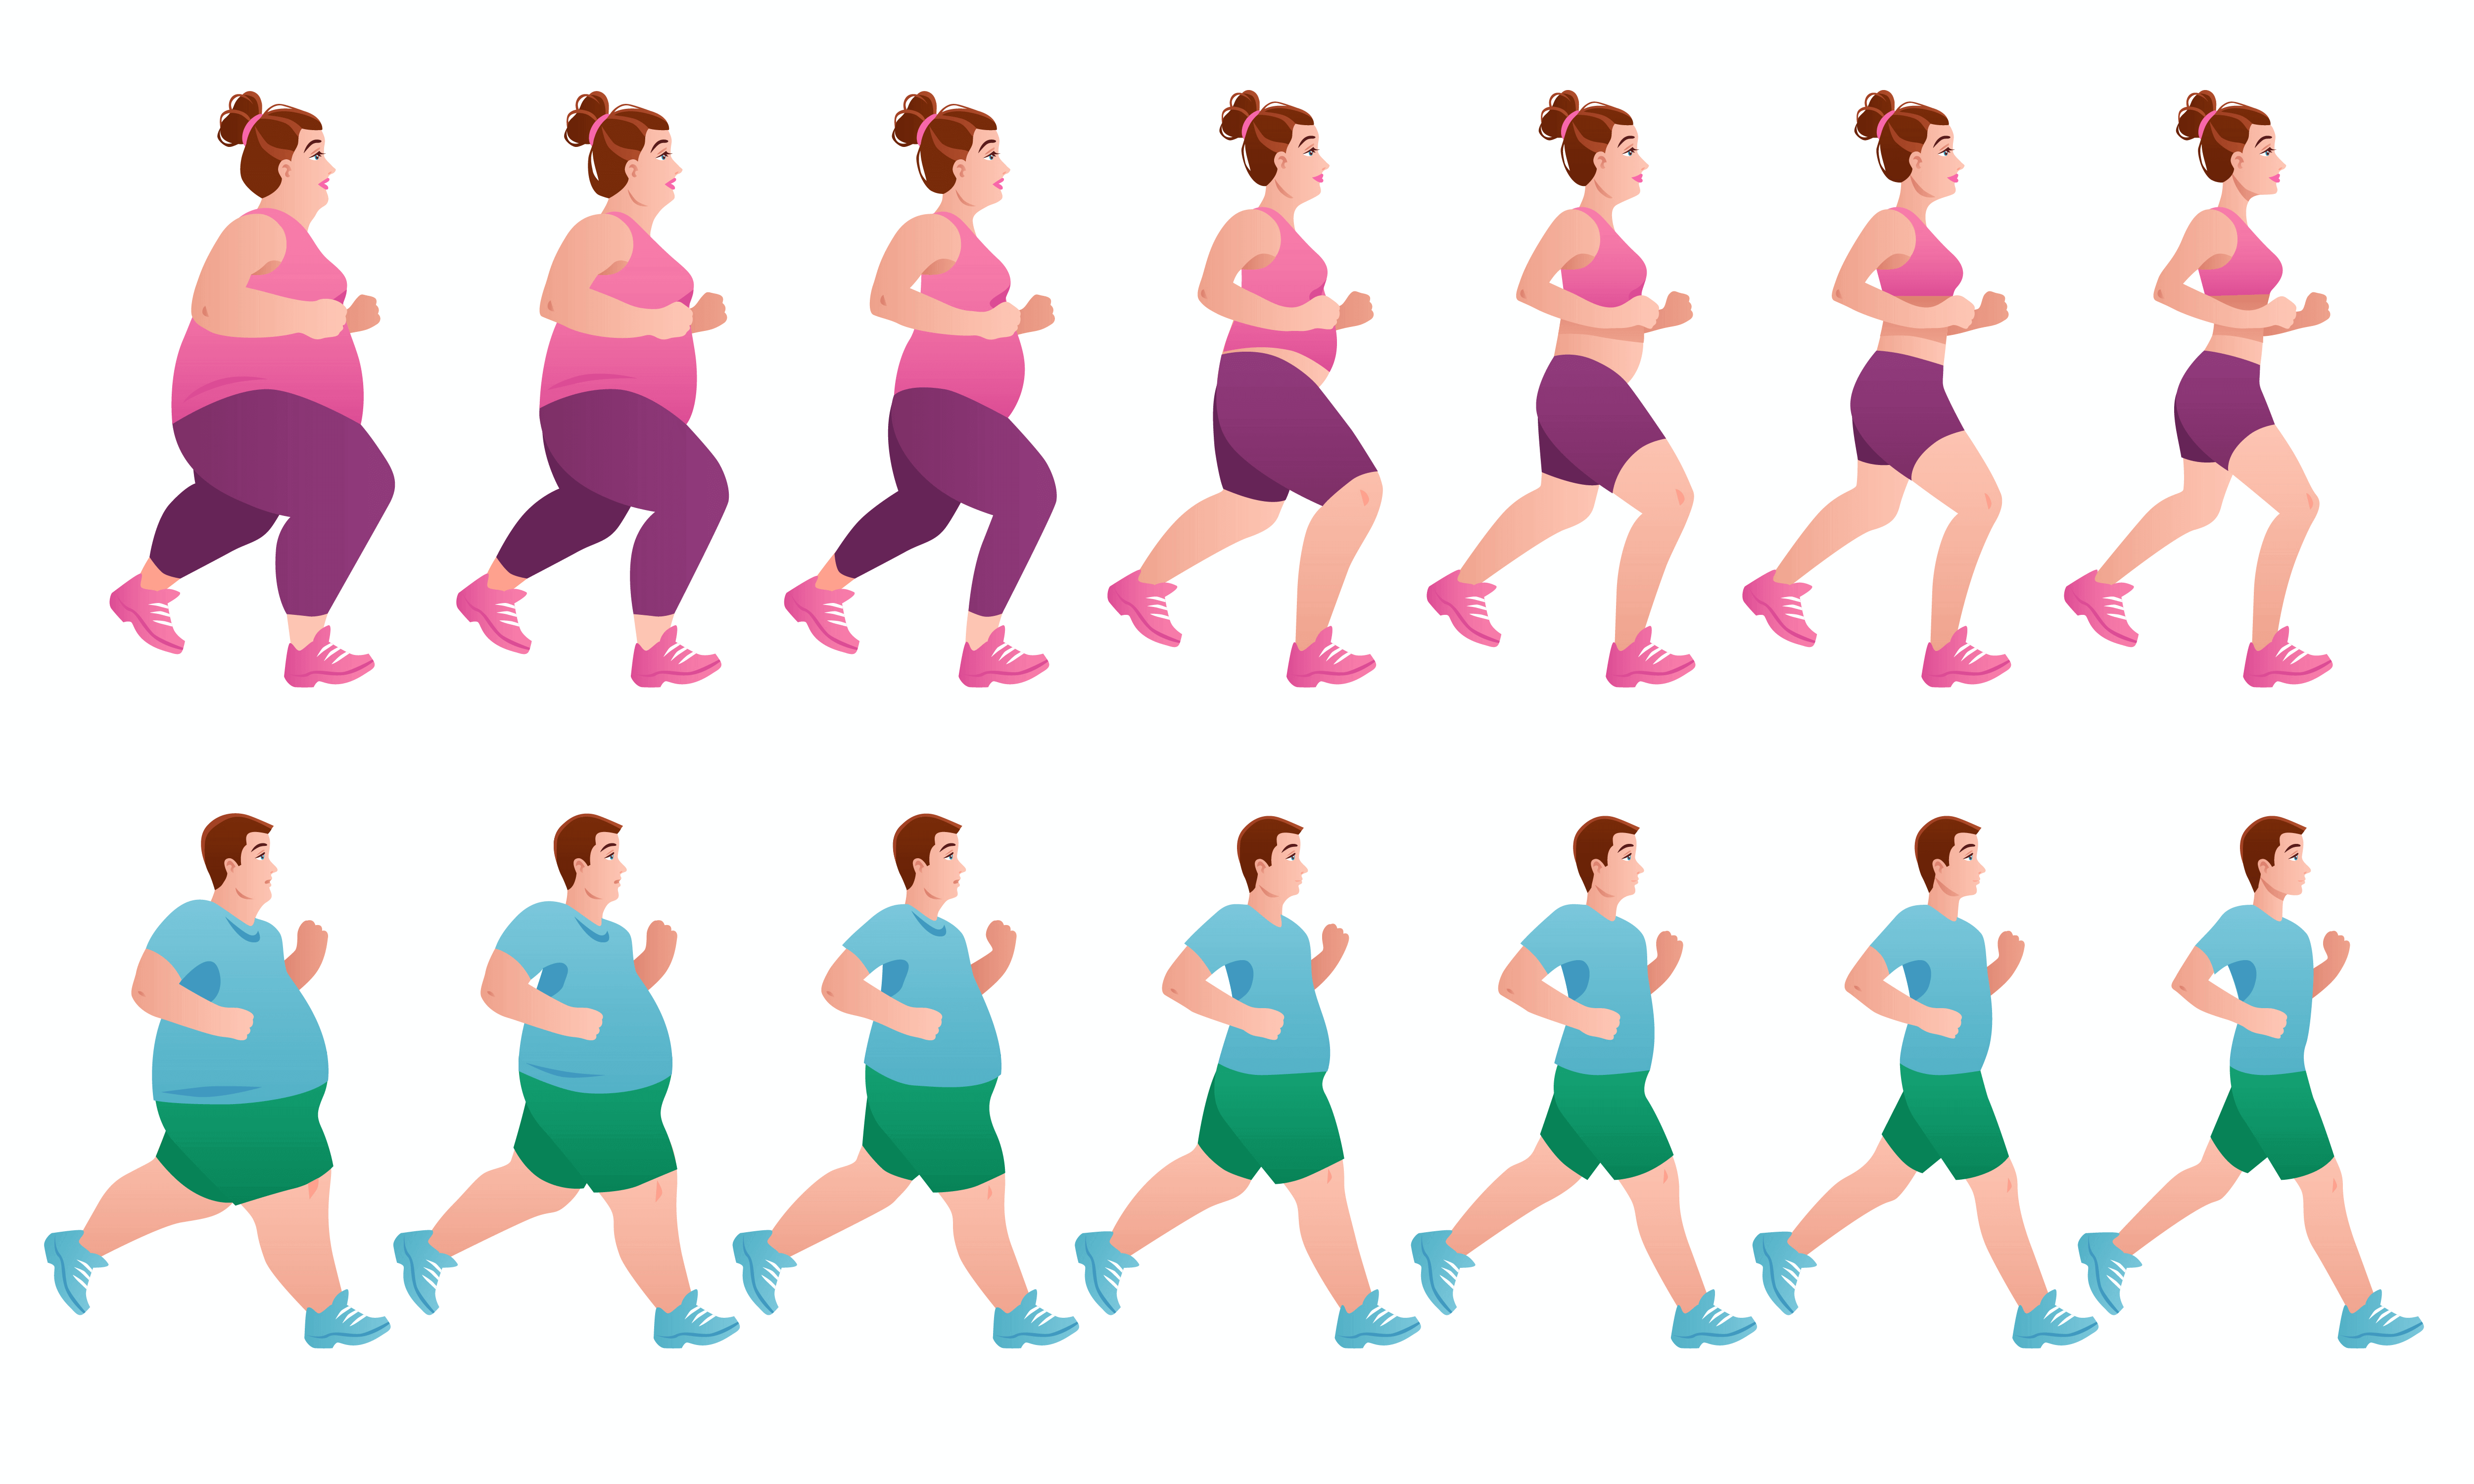
\includegraphics[width=.75\textwidth]{Images/NewIdeas/ExerciseTransformation.png}
    \caption{Example of how the virtual character could evolve as a result of training.}
    \label{fig:player_evolement}
\end{figure}

To register when the players are positioned at locations where they should earn points, geofencing will be used. Geofencing is based on defining areas on the map (illustrated in Figure \ref{fig:geofence}) where one can check whether or not the player is inside \citep{rouse_what_2016}. If the GPS location corresponds to a spot within the area, the player will be awarded points.

\begin{figure}[H]
    \centering
    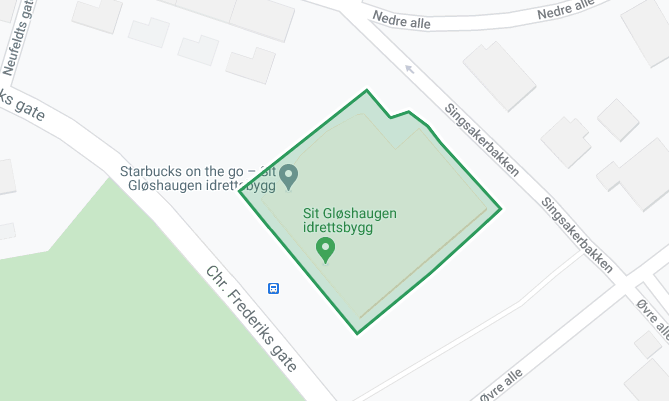
\includegraphics[width=.6\textwidth]{Images/NewIdeas/GeofenceExample.png}
    \caption{A geofence surrounding Sit Gløshaugen training center in Trondheim.}
    \label{fig:geofence}
\end{figure}

\textbf{Evaluation} \\
Hover is equivalent to Hold, categorized as an alternative game primarily based on two characteristics: Exploring alternative games genre by using gamification and using location data (GPS) in the gameplay.

The idea tries to increase people's well-being by motivating people to improve health, mental capabilities, socialize, and more. If the game concept is successful, it is valuable for both society and the individual.

Another important aspect when evaluating the concept is testability. Hover is easy to test because it has an extensive target group. Everyone owning a smartphone is a potential test subject. In addition to this, we think it will be easy to get people who agree to test this application because minimal extra time (despite answering a questionnaire) is required.


\subsection{Guess Where}
Guess Where is a challenge game, where players get to test how well they know their city. To earn points, players have to solve the challenges presented. A challenge consists of a street view picture where the player needs to figure out at which location it is captured; see Figure \ref{fig:street_view}). To complete the challenge, players must navigate to the correct site where their position is verified using GPS. The game is intended to reward completed challenges with fun facts about the area and in-game points.

\begin{wrapfigure}{r}{0.45\textwidth}
    \vspace*{-0.5\baselineskip}
    \centering
    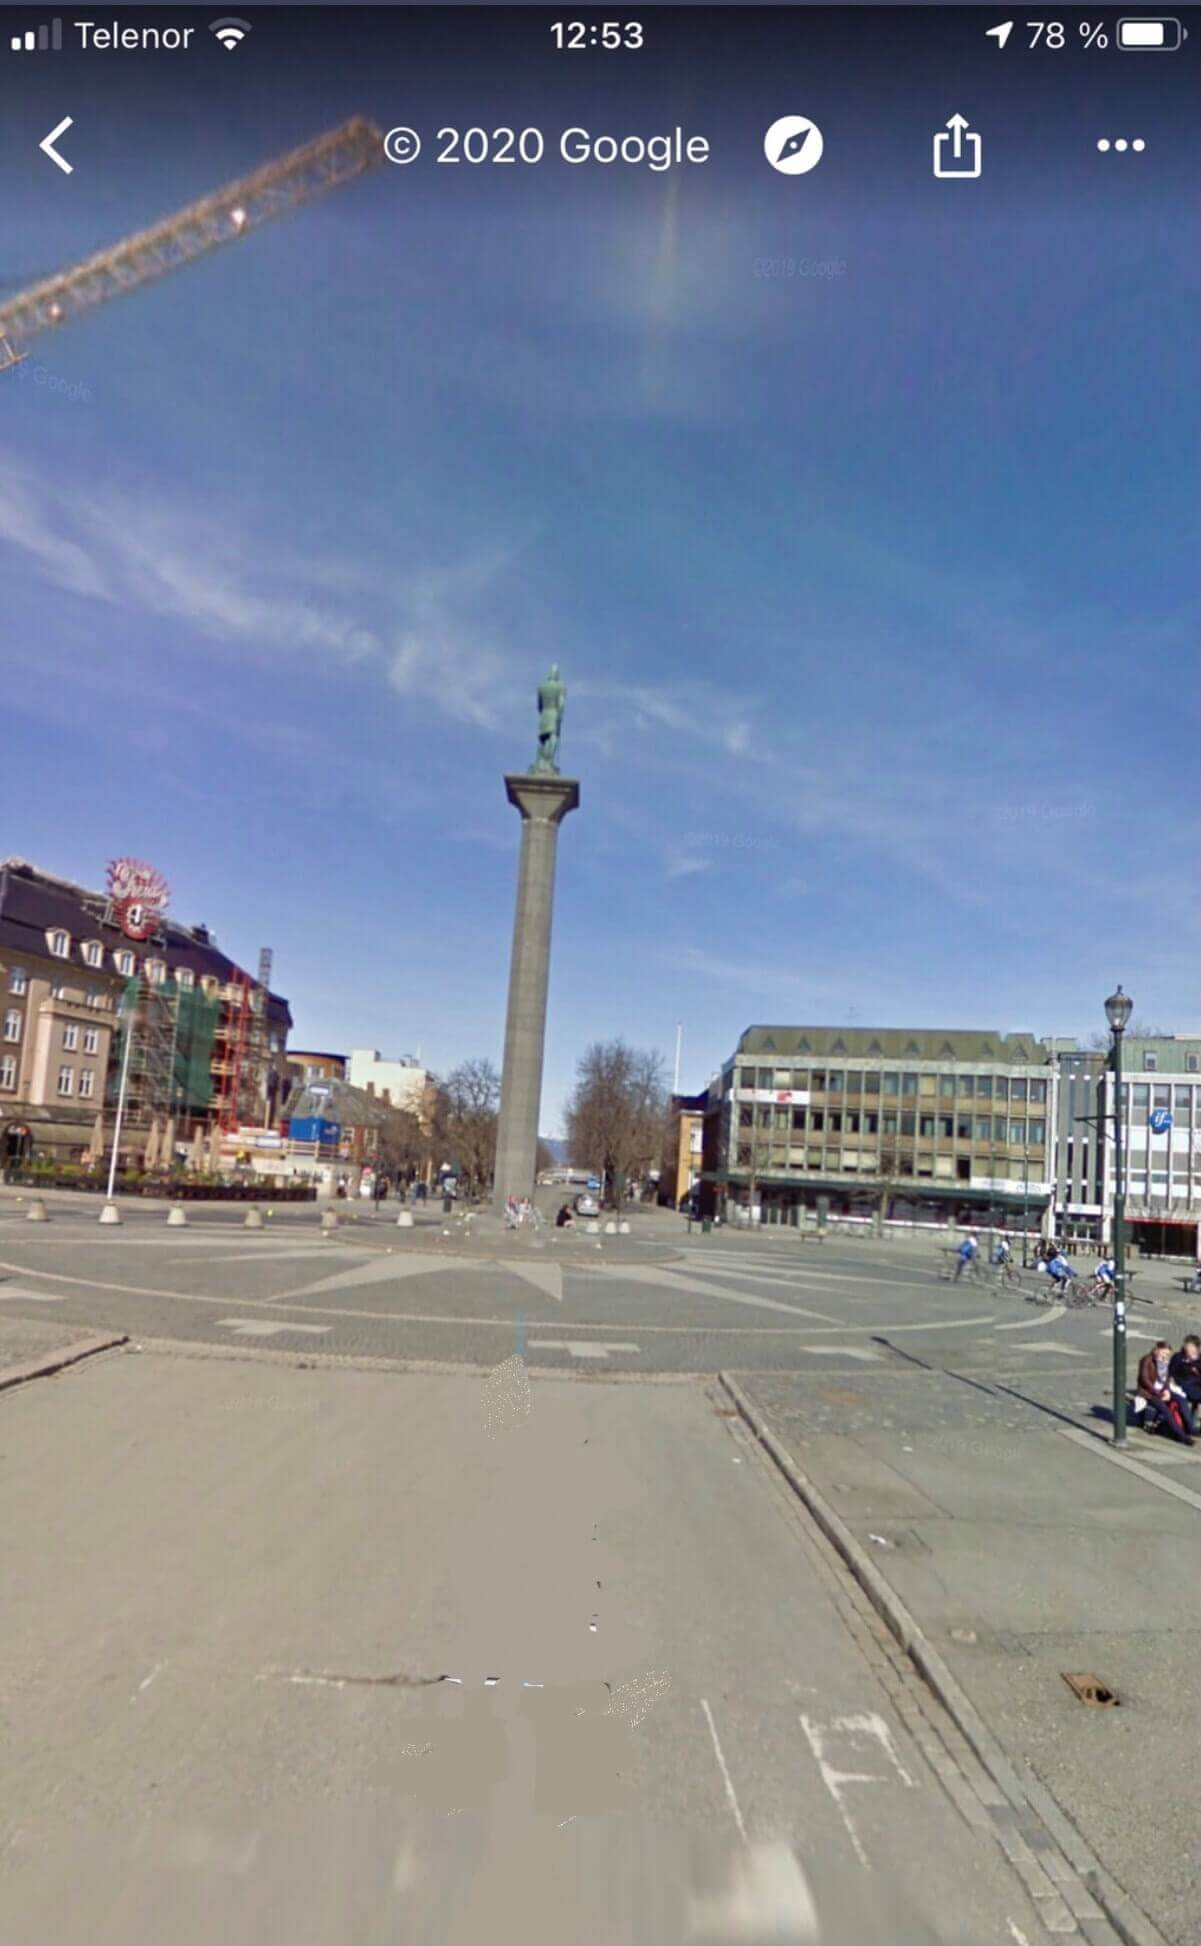
\includegraphics[width=0.35\textwidth]{Images/NewIdeas/StreetView.jpg}
    \caption{A street view photo of Trondheim Torg used as a hint in Guess Where.}
    \label{fig:street_view}
    \vspace*{-0.5\baselineskip}
\end{wrapfigure}

The concept can allow social interaction, both in the game and the real world. Players are encouraged to team up to boost their points. Accomplishments can also be shared with friends in a social feed inside the application. Social interaction through likes and comments can be motivating for further use. The concept is excellent for people that already have some knowledge of the city. However, by enabling hints, players can more easily complete the challenges.

\textbf{Evaluation}  \\
The concept fits into the alternative game model for several reasons, one being that the game is pervasive because it extends to the real world. For input, the game utilizes GPS for verifying a player’s location. In addition to this, the game fits into the domain of both entertainment and education. The game can also be categorized as the genre gamification that is considered an alternative game genre. 

The game concept is socially beneficial because it encourages social activities in the form of physical movement and collaboration while players can get to know the area better. One example where the game could be helpful is for educational purposes. Teenagers could team up and use this game for orientation in their gym classes. This approach could lead to improving cooperation skills while getting to know the city better. In terms of testability, this concept could easily, as in the example, be tested in a school class.

\subsection{Puzzle with Friends}
Puzzle with Friends is a game concept where the goal is to complete a puzzle together with your friends, as illustrated in Figure \ref{fig:friends_puzzle}. Each player is responsible for one piece they can move using their real-world position and rotating their mobile phone. All participants can watch the other players’ positions and the pattern they are supposed to puzzle in the application. The goal is to complete the puzzle, fit all the pieces in the correct spot, and rotate them correctly before the time is up. The number of pieces depends on how many players are collaborating on the same puzzle. Eight friends mean eight pieces, and so on. Thus the game will become increasingly challenging as the number of players increases. For the game to not become too easy, there should probably be a limitation on the minimum amount of players.

\begin{figure}[H]
    \centering
    \includegraphics[width=0.58\textwidth]{Images/NewIdeas/TeamworkPuzzleWithFriends.jpg}
    \caption{People collaborating to try to solve a puzzle in Puzzle with Friends.}
    \label{fig:friends_puzzle}
    \vspace*{-2\baselineskip}
\end{figure}

GPS location will be used to determine the player’s position. Because of the limitation in GPS accuracy \citep{merry_smartphone_2019}, a large outdoor area is required for the game to work as intended. Parks or football fields are good examples. Also, the more players that are included in the game, the more space is needed. Hence, there probably should exist a maximum number of players per game. The gameplay should also have a suitable mechanism for “snapping” pieces into the correct place when they are almost correctly aligned. This tool will make the game more delightful to play when minor location errors are present.

\begin{wrapfigure}{r}{0.4\textwidth}
    \centering
    
\includegraphics[width=0.35\textwidth]{Images/NewIdeas/Radar.png}
    \caption{A typical radar view. The “dots” will update every time the beam passes by.}
    \label{fig:radar_view}
    \vspace*{-1\baselineskip}
\end{wrapfigure}

As there probably will be some delay between the player’s movement and the application’s view, the gameplay needs to introduce some mechanism to hide this. One way to do this is by introducing some sort of radar view, see Figure \ref{fig:radar_view}, to illustrate that the other players’ position will only update at regular time intervals. 

\textbf{Evaluation}  \\
Puzzle with Friends is a typical alternative game because it uses alternative inputs to create a unique game concept. By utilizing the player’s position and heading in the real world to control the gameplay, the game is differentiated from other well-known puzzle games.

Developing the game should be manageable in the limited time we have during our master’s project. However, as mentioned above, inaccurate location data and real-time requirements may cause issues if not handled appropriately. Testing the application should be easy as long as we find some volunteers who agree to devote some hours of their day to test the application.


\subsection{Challenge Accepted}
Challenge Accepted is a social game that mixes social interaction with playful actions in the real world. The idea is based on a verbal game, often played among youths, called “\href{https://www.wikihow.com/Play-What-Are-the-Odds}{What are the odds?}". The game is usually played between two players where one player (A) gives the dare, and another player (B) receives it. The challenges often occur in the moment, for instance, “What are the odds of you asking that stranger to try his crutches?” To extend the concept a bit, players can publish challenges on a location that pops up when their friends walk by.
\begin{figure}[H]
    \centering
    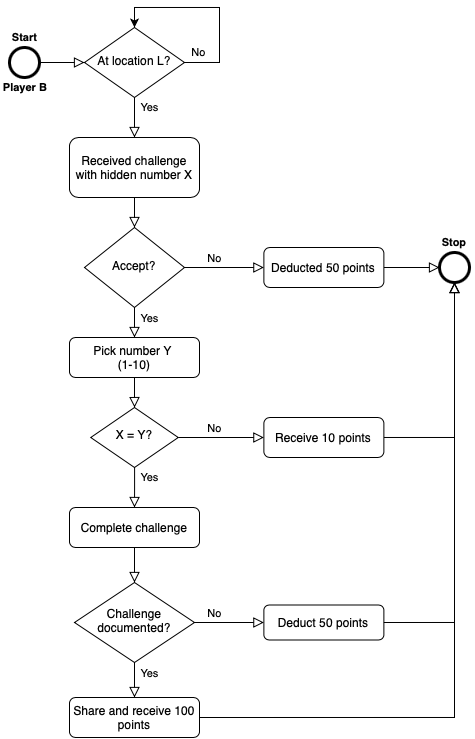
\includegraphics[width=.5\textwidth]{Images/NewIdeas/ChallengeAccepted.png}
    \caption{Flow chart illustrating a simplified game flow in Challenge Accepted.}
    \label{fig:challenge_accepted}
\end{figure}

Figure \ref{fig:challenge_accepted} shows a simplified game flow. The diagram is based on the following scenario: 

\begin{itemize}
    \item Player A adds a challenge to a location L, along with a number X between 1 and 10.
    \item A friend of player A, player B, walks by the location and receives a push notification.
    \item Player B has to either decline or accept the challenge. If the player chooses to decline, 50 points are lost. If the challenge is accepted, player B has to guess a number between 1 and 10.
    \item If the numbers are different, the player will not need to complete the challenge and receive 10 points for being courageous.
    \item However, if the numbers are equal, player B needs to do it. The challenge is considered completed when it is documented and shared in the application.
\end{itemize}

The goal of the game is to create spontaneous and surprising enjoyment between friends. The range of odds is set 1-10 because the risk of having to complete a challenge should not be too high nor too low. Also, challenges should be moderated to prevent them from being harmful. The game should include social interaction through likes and comments on in-game posts. Players should also be able to see their friends' game statistics and medals. Both these design elements are likely to have a positive effect on the competitiveness among friends.

\textbf{Evaluation}  \\
The idea classifies as alternative in the categories of input, game genre, and interaction. Besides location tracking, the concept also utilizes the camera for documenting challenges. Though the game is based on a verbal game, the game categorizes as gamification because players can be motivated through likes and comments on recent activities. 

The game is a pervasive game that utilizes location-tracking to create a bond between the virtual and the real world. The use of constant tracking of location contributes to the suspense of not knowing when, where, and what the next challenge will be. This suspense can also increase the players’ curiosity, and therefore their willingness to participate. 

The concept does not necessarily benefit society directly. However, it is a social game that has value for a smaller group of people. For testing purposes, it is advantageous to test the game on people with a pre-existing relationship, to enhance the players’ motivation to complete the challenges.


\subsection{Secret Posts}
Secret Posts is an extension and gamification concept based on the social app \href{https://jodel.com}{Jodel}, where players can share anonymous posts in their city. Since the posts are anonymous, people tend to post their secrets, embarrassing stories, and pictures. Our concept involves posting digital notes, drawings, or images in the real world, which only can be seen using Augmented Reality (AR) technology. All players can share posts attached to the location where they are posted. An example can be a sticky-note with a secret message lying on a table in a cafeteria. To find posts, players use a map to locate nearby ones, as seen in Figure \ref{fig:secret_notes_map}. Although the posts’ location is visible on the map, the content is only available through the mobile camera. As illustrated in Figure \ref{fig:secret_notes_camera}, players use their mobile camera to read new posts in their current area. Since the posts only are visible to the players, a secret society is created where “only those who know, know.”

\begin{figure}[H]
    \begin{minipage}{.48\textwidth}
        \centering
        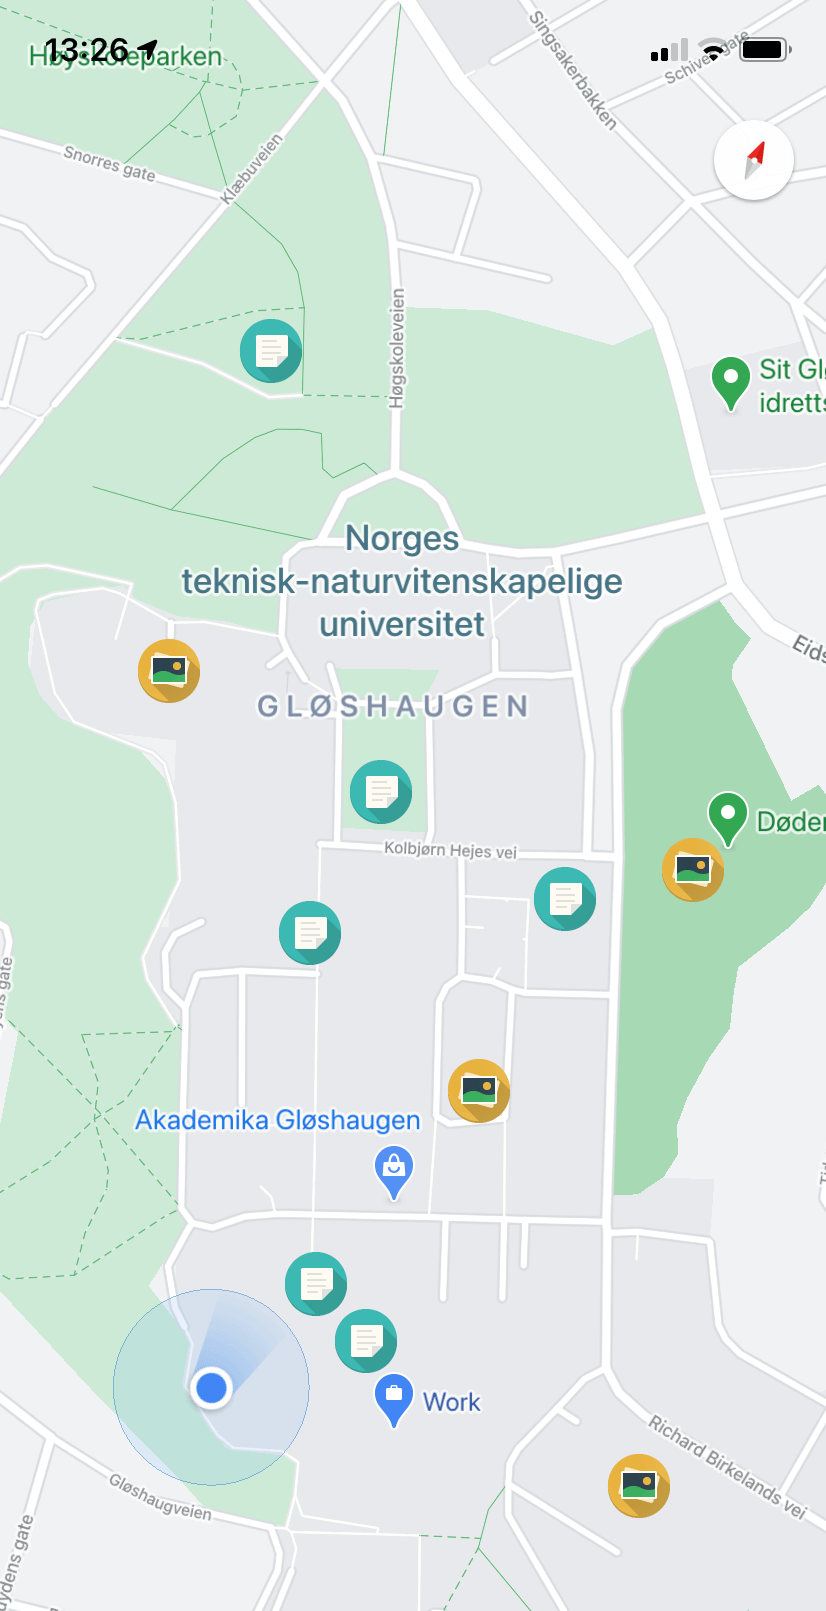
\includegraphics[width=.8\textwidth]{Images/NewIdeas/SecretNotesMap.png}
        \captionof{figure}{The map-view in Secret Notes showing nearby posts.}
        \label{fig:secret_notes_map}
        \end{minipage}
        \hspace*{0.5\baselineskip}
        \begin{minipage}{.48\textwidth}
        \centering
        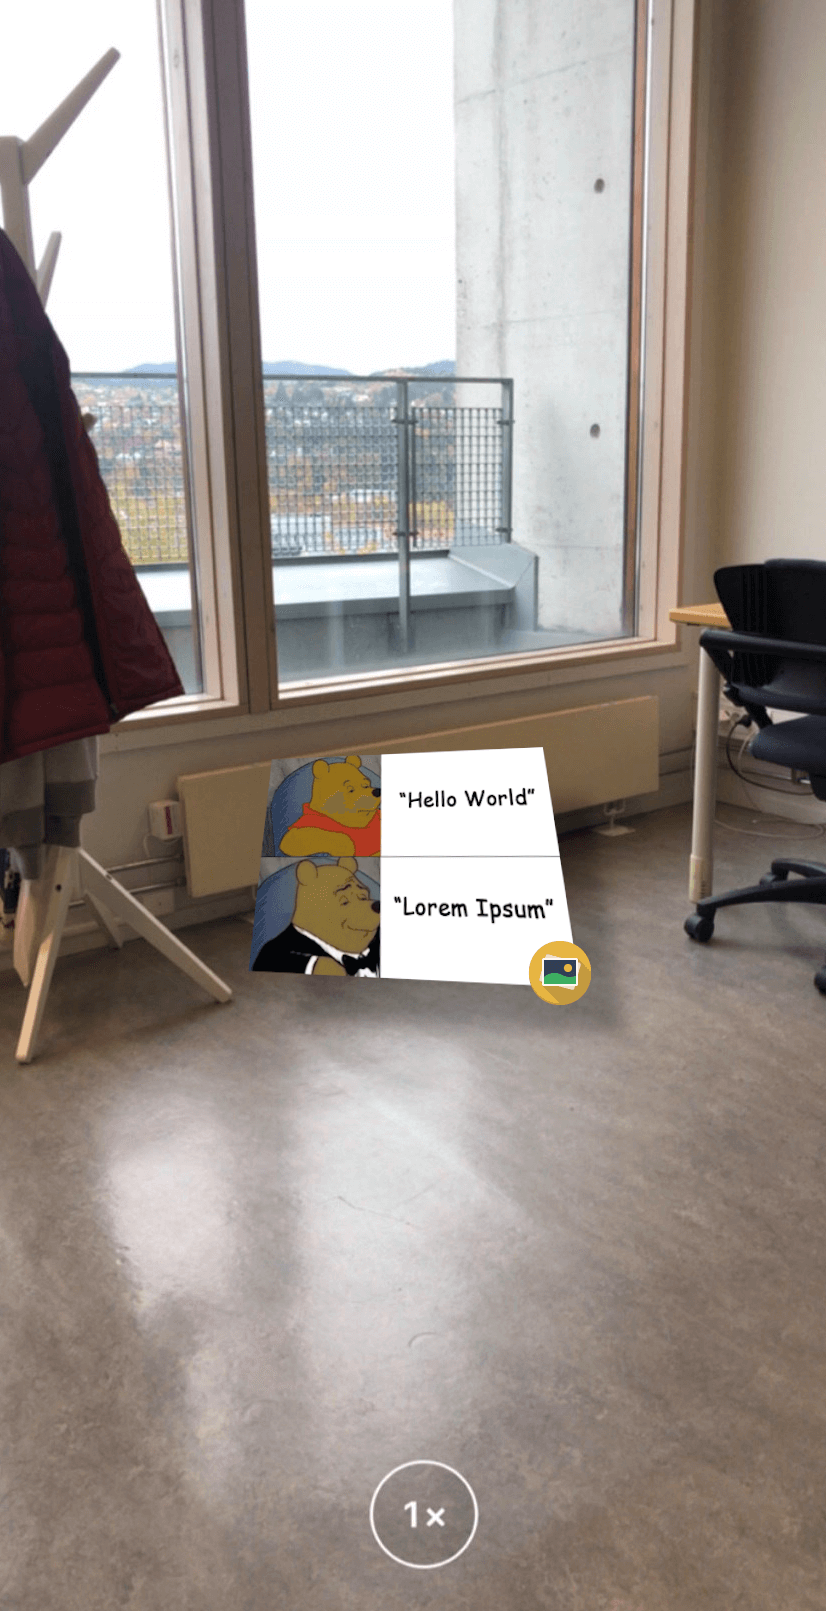
\includegraphics[width=.8\textwidth]{Images/NewIdeas/SecretNotesCamera.png}
        \captionof{figure}{AR view of the content of a note found in Secret Notes.}
        \label{fig:secret_notes_camera}
    \end{minipage}
\end{figure}


\textbf{Evaluation}  \\
The concept is alternative in its usage of input, output, game genre, and concept. The game uses the phone’s camera as input, which it uses to project a note, image, or drawing. This usage of AR is not too common as of 2021; hence the input method is alternative. The concept is also alternative because it uses location to attach anonymous posts. Tangible objects like notes, posters, and graffiti are not unfamiliar in the real world. However, the fact that the posts are only visible for those who search for them makes the game alternative.

The concept is suited for AR glasses and as a mobile application. The benefit of using AR glasses is that the users can walk around and discover notes without actively looking. However, in terms of testability, the AR glasses approach has a clear disadvantage compared to a mobile application in terms of equipment available and the project’s time scope. As a mobile application, the concept should be straightforward to develop and test.


\subsection{Free Ticket to Ride}
The purpose of this game concept is to incentivize having a valid ticket when using public transport. The idea is to create an application that gamifies the ticket system used on public transport. It could be adopted as an alternative or addition to normal ticket controls used today.

The application will need to integrate with the existing application to validate tickets. People who have paid for a valid ticket will be given points in the game when traveling. After earning a set amount of points, the user can “purchase” free items or get discounts. One suggestion is to use free or discounted single tickets as rewards. For example, twenty rides with a valid ticket could qualify for one free ticket. A prerequisite for this is, of course, a partnership with a public transport company, such as AtB in Trondheim. Even though the concept is invented and conceptualized based on the public transport system in Trondheim, the same ideas could be adopted in other cities with similar ticket systems as well.

The application can communicate with a Bluetooth access point to check if a user is located in a public transport vehicle and award points accordingly (illustrated in Figure \ref{fig:people_on_the_bus}). A secondary registration option using the camera and scanning QR codes could also be an alternative to situations where the bus does not have a Bluetooth access point, or the user does not consent to Bluetooth usage.

\begin{figure}[H]
    \centering
    
\includegraphics[width=0.75\textwidth]{Images/NewIdeas/PeopleOnTheBus.png}
    \caption{Illustration of people using Free Ticket to Ride on public transport.}
    \label{fig:people_on_the_bus}
\end{figure}


\textbf{Evaluation}  \\
Free ticket to ride is an alternative game concept because it uses Bluetooth as input. Additionally, the idea explores the gamification genre. By the definition of an alternative game (Chapter \ref{chap:what_is_alternative_game}), these two characteristics define this as alternative.

The game introduces a fun way of validating the user’s ticket when using public transport, which could lead to fewer fare evasions. Getting more people to pay for their ride will result in more income for the public transport company, which can improve the service. 

One of the main problems with this idea is the need for tight integration with the current public transport company. The concept requires integration with the ticket system to check the validity of the ticket.


\subsection{Comparison of Game Concepts}
Similarly, as in Chapter \ref{chap:comparison_of_existing_games}, when existing alternative game concepts were presented, our new ideas are compared using the alternative games model described in Chapter \ref{chap:design_an_enjoyable_game}. All of the game concepts are categorized using the six characteristics of alternative games.

\begin{table}[H]
    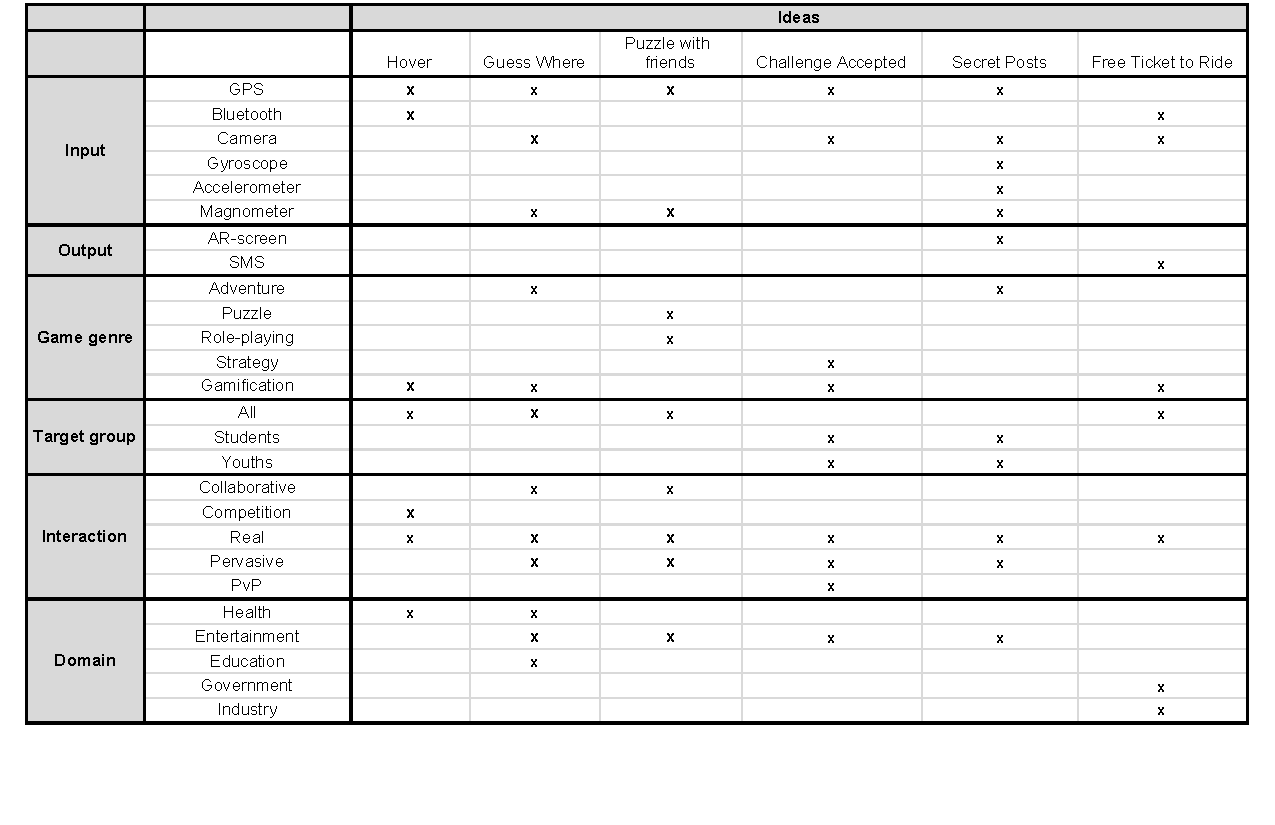
\includegraphics[width=1\textwidth]{Images/Models/OurConcepts.pdf}
    \vspace*{-3\baselineskip}
    \caption{Comparison of Game Concepts}
   \label{tab:new_ideas_comparison}
\end{table}

In contrast to the comparison of existing alternative games, our new concepts have a lot in common and often tick the same boxes in the model, as seen in Table \ref{tab:new_ideas_comparison}. The existing alternative games were picked partly based on their difference, so this is expected. As mentioned at the beginning of this chapter, we limited ourselves to concepts based on the mobile platform. Thus all the games are restricted to input and output provided by a smartphone. For input, a selection of the available sensors in a mobile phone has been used. GPS for location tracking is the most common, with four out of six concepts using it. Output possibilities on a mobile phone are more limited. There are not a lot of possible outputs that we would categorize as alternative. Two exceptions are found in Secret Posts and Free Ticket to Ride. These games respectively use an AR screen for displaying the notes and SMS to verify users and notify them of important events.

One of the most notable similarities in the comparison is the use of gamification as the game genre. This similarity is related to our goal in the project; trying to do something socially beneficial. We found it easier to invent gamification ideas with a socially beneficial purpose than other genres.

As we also described in our motivation (Chapter \ref{chap:motivation}), an influential factor when inventing ideas was trying to reach as many users as possible. Therefore, the applications are usually targeted at all user types. However, two of the concepts have youths and students as the primary target group.

The last two categories address interaction and domain. In the interaction category, we see that all games include aspects of the real-world. Four of the games are also pervasive, meaning that they mix reality and virtuality. The most common domain in the applications is entertainment, with four of six applications characterized as it. Hover and Free Ticket to Ride are the only ones that are not categorized as entertainment. They fall into the health and government/industry domain, respectively.

\subsection{Summary}
In this chapter, our ideas for new alternative game concepts were described. A brief description of all of the concepts and an evaluation of them were conducted. We looked at why the concepts can be categorized as alternative games and how they fit with our goal and motivation in the project. Additionally, we looked at the testability of the ideas. Last, we compared the concepts and looked at differences using the alternative games model defined earlier. The next chapter will use these observations and evaluations when we will choose the concept we are going to develop in our master’s thesis.

\clearpage